\documentclass[aspectratio=169,11pt]{beamer}
% ==========================================================================
%  KSA lecture-slide theme  =  stock beamer "Boadilla"  +  KSA colour theme
%  brand colours sampled from the official KSA symbol mark:
%    Deep Prussian Blue  #2E3192   (지성 - intellect)
%    Golden Gray         #D6CBB1   (감성 - sensibility)
%  Engine: XeLaTeX.  Usage:
%    \documentclass[aspectratio=169,11pt]{beamer}
%    % ==========================================================================
%  KSA lecture-slide theme  =  stock beamer "Boadilla"  +  KSA colour theme
%  brand colours sampled from the official KSA symbol mark:
%    Deep Prussian Blue  #2E3192   (지성 - intellect)
%    Golden Gray         #D6CBB1   (감성 - sensibility)
%  Engine: XeLaTeX.  Usage:
%    \documentclass[aspectratio=169,11pt]{beamer}
%    % ==========================================================================
%  KSA lecture-slide theme  =  stock beamer "Boadilla"  +  KSA colour theme
%  brand colours sampled from the official KSA symbol mark:
%    Deep Prussian Blue  #2E3192   (지성 - intellect)
%    Golden Gray         #D6CBB1   (감성 - sensibility)
%  Engine: XeLaTeX.  Usage:
%    \documentclass[aspectratio=169,11pt]{beamer}
%    \input{../theme/ksa-theme.tex}
% ==========================================================================

\usepackage{fontspec}
\usepackage{amsmath,amssymb}
\usepackage{graphicx}
\graphicspath{{figs/}{../figs/}}
\usepackage{booktabs}
\usepackage{listings}

% ---- fonts (no ctex/xeCJK on this box -> fontspec drives CJK directly) -----
\defaultfontfeatures{Ligatures=TeX}
\setmainfont{Noto Sans CJK KR}
\setsansfont{Noto Sans CJK KR}
\setmonofont{Noto Sans Mono CJK KR}[Scale=0.92]

% ---- base theme: stock Boadilla ------------------------------------------
\usetheme{Boadilla}
\usefonttheme{professionalfonts}
\setbeamertemplate{navigation symbols}{}

% ---- KSA colour theme (recolour the stock theme) --------------------------
\definecolor{ksablue}{HTML}{2E3192}
\definecolor{ksabluedk}{HTML}{20226A}
\definecolor{ksagold}{HTML}{D6CBB1}
\definecolor{ksagolddk}{HTML}{A9976B}
\definecolor{ksared}{HTML}{C0392B}
\definecolor{ksagray}{HTML}{5B5B5B}

\setbeamercolor{structure}{fg=ksablue}
\setbeamercolor{alerted text}{fg=ksared}

\setbeamercolor{palette primary}{fg=white,           bg=ksablue}
\setbeamercolor{palette secondary}{fg=white,         bg=ksablue!85!black}
\setbeamercolor{palette tertiary}{fg=white,          bg=ksabluedk}
\setbeamercolor{titlelike}{fg=ksablue}
\setbeamercolor{frametitle}{fg=ksablue,bg=}
\setbeamercolor{title}{fg=ksablue}
\setbeamercolor{author}{fg=ksagray}
\setbeamercolor{institute}{fg=ksagray}
\setbeamercolor{block title}{fg=white,bg=ksablue}
\setbeamercolor{block body}{fg=black!85,bg=ksablue!6}
\setbeamercolor{item}{fg=ksablue}
\setbeamercolor{section in toc}{fg=black!85}

\setbeamerfont{frametitle}{series=\bfseries}
\setbeamerfont{title}{series=\bfseries}

% ---- footline:  KSA mark | "Made by ..." | n / N   (matches reference) ----
\newcommand{\ksacredit}{Made by Sumin Han \,\textperiodcentered\, suminhan@ksa.hs.kr}
\setbeamertemplate{footline}{%
  \hbox{%
    \begin{beamercolorbox}[wd=.18\paperwidth,ht=2.6ex,dp=1.5ex,leftskip=1.1em]{}%
      \raisebox{-0.35ex}{
\includegraphics[height=2.0ex]{ksa-logo.png}}%
    \end{beamercolorbox}%
    \begin{beamercolorbox}[wd=.64\paperwidth,ht=2.6ex,dp=1.5ex,center]{}%
      {\scriptsize\color{ksagray}\ksacredit}%
    \end{beamercolorbox}%
    \begin{beamercolorbox}[wd=.18\paperwidth,ht=2.6ex,dp=1.5ex,rightskip=1.1em]{}%
      \hfill{\scriptsize\color{ksablue}\insertframenumber\,/\,\inserttotalframenumber}%
    \end{beamercolorbox}%
  }%
  \vskip2pt
}

% ---- section divider: stock \sectionpage, KSA-coloured -------------------
\setbeamertemplate{section page}{%
  \begingroup\centering
    {\color{ksagolddk}\rule{0.16\paperwidth}{1pt}}\par\vskip1.0em
    {\usebeamerfont{title}\color{ksablue}\insertsectionhead\par}\vskip1.0em
    {\color{ksagolddk}\rule{0.16\paperwidth}{1pt}}\par
  \endgroup
}
\AtBeginSection[]{\begin{frame}[plain,noframenumbering]\vfill\sectionpage\vfill\end{frame}}

% ---- code listings ------------------------------------------------------------
\lstdefinestyle{ksa}{%
  basicstyle=\ttfamily\scriptsize,
  keywordstyle=\color{ksablue}\bfseries,
  commentstyle=\color{ksagray}\itshape,
  stringstyle=\color{ksagolddk},
  numberstyle=\tiny\color{ksagray},
  backgroundcolor=\color{ksablue!6},
  frame=leftline, framerule=1.4pt, rulecolor=\color{ksablue},
  xleftmargin=1em, aboveskip=0.8em, belowskip=0.4em,
  showstringspaces=false, breaklines=true, language=Python,
}
\lstset{style=ksa}

% ---- handy macros -----------------------------------------------------------
\newcommand{\kb}[1]{\textbf{\color{ksablue}#1}}   % blue keyword
\newcommand{\kq}[1]{\textbf{\color{ksared}#1}}    % red key-question

% ==========================================================================

\usepackage{fontspec}
\usepackage{amsmath,amssymb}
\usepackage{graphicx}
\graphicspath{{figs/}{../figs/}}
\usepackage{booktabs}
\usepackage{listings}

% ---- fonts (no ctex/xeCJK on this box -> fontspec drives CJK directly) -----
\defaultfontfeatures{Ligatures=TeX}
\setmainfont{Noto Sans CJK KR}
\setsansfont{Noto Sans CJK KR}
\setmonofont{Noto Sans Mono CJK KR}[Scale=0.92]

% ---- base theme: stock Boadilla ------------------------------------------
\usetheme{Boadilla}
\usefonttheme{professionalfonts}
\setbeamertemplate{navigation symbols}{}

% ---- KSA colour theme (recolour the stock theme) --------------------------
\definecolor{ksablue}{HTML}{2E3192}
\definecolor{ksabluedk}{HTML}{20226A}
\definecolor{ksagold}{HTML}{D6CBB1}
\definecolor{ksagolddk}{HTML}{A9976B}
\definecolor{ksared}{HTML}{C0392B}
\definecolor{ksagray}{HTML}{5B5B5B}

\setbeamercolor{structure}{fg=ksablue}
\setbeamercolor{alerted text}{fg=ksared}

\setbeamercolor{palette primary}{fg=white,           bg=ksablue}
\setbeamercolor{palette secondary}{fg=white,         bg=ksablue!85!black}
\setbeamercolor{palette tertiary}{fg=white,          bg=ksabluedk}
\setbeamercolor{titlelike}{fg=ksablue}
\setbeamercolor{frametitle}{fg=ksablue,bg=}
\setbeamercolor{title}{fg=ksablue}
\setbeamercolor{author}{fg=ksagray}
\setbeamercolor{institute}{fg=ksagray}
\setbeamercolor{block title}{fg=white,bg=ksablue}
\setbeamercolor{block body}{fg=black!85,bg=ksablue!6}
\setbeamercolor{item}{fg=ksablue}
\setbeamercolor{section in toc}{fg=black!85}

\setbeamerfont{frametitle}{series=\bfseries}
\setbeamerfont{title}{series=\bfseries}

% ---- footline:  KSA mark | "Made by ..." | n / N   (matches reference) ----
\newcommand{\ksacredit}{Made by Sumin Han \,\textperiodcentered\, suminhan@ksa.hs.kr}
\setbeamertemplate{footline}{%
  \hbox{%
    \begin{beamercolorbox}[wd=.18\paperwidth,ht=2.6ex,dp=1.5ex,leftskip=1.1em]{}%
      \raisebox{-0.35ex}{
\includegraphics[height=2.0ex]{ksa-logo.png}}%
    \end{beamercolorbox}%
    \begin{beamercolorbox}[wd=.64\paperwidth,ht=2.6ex,dp=1.5ex,center]{}%
      {\scriptsize\color{ksagray}\ksacredit}%
    \end{beamercolorbox}%
    \begin{beamercolorbox}[wd=.18\paperwidth,ht=2.6ex,dp=1.5ex,rightskip=1.1em]{}%
      \hfill{\scriptsize\color{ksablue}\insertframenumber\,/\,\inserttotalframenumber}%
    \end{beamercolorbox}%
  }%
  \vskip2pt
}

% ---- section divider: stock \sectionpage, KSA-coloured -------------------
\setbeamertemplate{section page}{%
  \begingroup\centering
    {\color{ksagolddk}\rule{0.16\paperwidth}{1pt}}\par\vskip1.0em
    {\usebeamerfont{title}\color{ksablue}\insertsectionhead\par}\vskip1.0em
    {\color{ksagolddk}\rule{0.16\paperwidth}{1pt}}\par
  \endgroup
}
\AtBeginSection[]{\begin{frame}[plain,noframenumbering]\vfill\sectionpage\vfill\end{frame}}

% ---- code listings ------------------------------------------------------------
\lstdefinestyle{ksa}{%
  basicstyle=\ttfamily\scriptsize,
  keywordstyle=\color{ksablue}\bfseries,
  commentstyle=\color{ksagray}\itshape,
  stringstyle=\color{ksagolddk},
  numberstyle=\tiny\color{ksagray},
  backgroundcolor=\color{ksablue!6},
  frame=leftline, framerule=1.4pt, rulecolor=\color{ksablue},
  xleftmargin=1em, aboveskip=0.8em, belowskip=0.4em,
  showstringspaces=false, breaklines=true, language=Python,
}
\lstset{style=ksa}

% ---- handy macros -----------------------------------------------------------
\newcommand{\kb}[1]{\textbf{\color{ksablue}#1}}   % blue keyword
\newcommand{\kq}[1]{\textbf{\color{ksared}#1}}    % red key-question

% ==========================================================================

\usepackage{fontspec}
\usepackage{amsmath,amssymb}
\usepackage{graphicx}
\graphicspath{{figs/}{../figs/}}
\usepackage{booktabs}
\usepackage{listings}

% ---- fonts (no ctex/xeCJK on this box -> fontspec drives CJK directly) -----
\defaultfontfeatures{Ligatures=TeX}
\setmainfont{Noto Sans CJK KR}
\setsansfont{Noto Sans CJK KR}
\setmonofont{Noto Sans Mono CJK KR}[Scale=0.92]

% ---- base theme: stock Boadilla ------------------------------------------
\usetheme{Boadilla}
\usefonttheme{professionalfonts}
\setbeamertemplate{navigation symbols}{}

% ---- KSA colour theme (recolour the stock theme) --------------------------
\definecolor{ksablue}{HTML}{2E3192}
\definecolor{ksabluedk}{HTML}{20226A}
\definecolor{ksagold}{HTML}{D6CBB1}
\definecolor{ksagolddk}{HTML}{A9976B}
\definecolor{ksared}{HTML}{C0392B}
\definecolor{ksagray}{HTML}{5B5B5B}

\setbeamercolor{structure}{fg=ksablue}
\setbeamercolor{alerted text}{fg=ksared}

\setbeamercolor{palette primary}{fg=white,           bg=ksablue}
\setbeamercolor{palette secondary}{fg=white,         bg=ksablue!85!black}
\setbeamercolor{palette tertiary}{fg=white,          bg=ksabluedk}
\setbeamercolor{titlelike}{fg=ksablue}
\setbeamercolor{frametitle}{fg=ksablue,bg=}
\setbeamercolor{title}{fg=ksablue}
\setbeamercolor{author}{fg=ksagray}
\setbeamercolor{institute}{fg=ksagray}
\setbeamercolor{block title}{fg=white,bg=ksablue}
\setbeamercolor{block body}{fg=black!85,bg=ksablue!6}
\setbeamercolor{item}{fg=ksablue}
\setbeamercolor{section in toc}{fg=black!85}

\setbeamerfont{frametitle}{series=\bfseries}
\setbeamerfont{title}{series=\bfseries}

% ---- footline:  KSA mark | "Made by ..." | n / N   (matches reference) ----
\newcommand{\ksacredit}{Made by Sumin Han \,\textperiodcentered\, suminhan@ksa.hs.kr}
\setbeamertemplate{footline}{%
  \hbox{%
    \begin{beamercolorbox}[wd=.18\paperwidth,ht=2.6ex,dp=1.5ex,leftskip=1.1em]{}%
      \raisebox{-0.35ex}{
\includegraphics[height=2.0ex]{ksa-logo.png}}%
    \end{beamercolorbox}%
    \begin{beamercolorbox}[wd=.64\paperwidth,ht=2.6ex,dp=1.5ex,center]{}%
      {\scriptsize\color{ksagray}\ksacredit}%
    \end{beamercolorbox}%
    \begin{beamercolorbox}[wd=.18\paperwidth,ht=2.6ex,dp=1.5ex,rightskip=1.1em]{}%
      \hfill{\scriptsize\color{ksablue}\insertframenumber\,/\,\inserttotalframenumber}%
    \end{beamercolorbox}%
  }%
  \vskip2pt
}

% ---- section divider: stock \sectionpage, KSA-coloured -------------------
\setbeamertemplate{section page}{%
  \begingroup\centering
    {\color{ksagolddk}\rule{0.16\paperwidth}{1pt}}\par\vskip1.0em
    {\usebeamerfont{title}\color{ksablue}\insertsectionhead\par}\vskip1.0em
    {\color{ksagolddk}\rule{0.16\paperwidth}{1pt}}\par
  \endgroup
}
\AtBeginSection[]{\begin{frame}[plain,noframenumbering]\vfill\sectionpage\vfill\end{frame}}

% ---- code listings ------------------------------------------------------------
\lstdefinestyle{ksa}{%
  basicstyle=\ttfamily\scriptsize,
  keywordstyle=\color{ksablue}\bfseries,
  commentstyle=\color{ksagray}\itshape,
  stringstyle=\color{ksagolddk},
  numberstyle=\tiny\color{ksagray},
  backgroundcolor=\color{ksablue!6},
  frame=leftline, framerule=1.4pt, rulecolor=\color{ksablue},
  xleftmargin=1em, aboveskip=0.8em, belowskip=0.4em,
  showstringspaces=false, breaklines=true, language=Python,
}
\lstset{style=ksa}

% ---- handy macros -----------------------------------------------------------
\newcommand{\kb}[1]{\textbf{\color{ksablue}#1}}   % blue keyword
\newcommand{\kq}[1]{\textbf{\color{ksared}#1}}    % red key-question


\title{Block A 캡스톤: 팀 프로젝트와 총정리}
\subtitle{팀 프로젝트 4주 파이프라인 · Peer-Review · 중간고사 대비 총정리}
\author{Machine Learning 1 \,\textperiodcentered\, 8주차}
\institute{한국과학영재학교 (KSA)}
\date{Chapter 8}

\begin{document}

% ===== title =====
\begin{frame}[plain,noframenumbering]\titlepage\end{frame}

% ===== roadmap of this week =====
\begin{frame}{이번 주차 개요}
  \begin{itemize}
    \item \kb{8.1 팀 프로젝트} --- 4주 파이프라인으로 정형 데이터에
      Ch.\,2--7 모델을 적용. \kq{산출물은 높은 성능이 아니라
      ``성능 숫자를 정직하게 얻은 절차''.}
    \item \kb{8.2 Peer-Review} --- 이번엔 네가 심사위원. 체크리스트로
      두 팀을 검토하고, 장·절을 명시한 반박 가능한 질문을 쓴다.
    \item \kb{8.3 중간고사 대비 총정리} --- 유도 템플릿 3가지를 종이에
      재현하고, 장별 핵심 질문으로 자가진단.
  \end{itemize}
  \vskip0.6em
  \begin{block}{이번 장을 마치면}
    모델·지표·전처리·분할을 스스로 골라 근거지을 수 있고,
    3분할·베이스라인·``test 한 번'' 절차를 실제로 수행해
    보고서·발표로 제시할 수 있다.
  \end{block}
  \vskip0.4em
  \begin{center}
  \kq{같은 절차를 세 가지 언어(코드, 보고서, 리뷰)로 말할 수 있어야
       이 프로젝트가 끝난 것이다.}
  \end{center}
\end{frame}

\section{8.1 팀 프로젝트: 데이터 선정부터 발표까지}

\begin{frame}{왜 지금 프로젝트를 하는가}
  \begin{columns}[T]
    \begin{column}{0.55\textwidth}
      \begin{itemize}
        \item 트리 기반 모델(Ch.\,7)까지 끝내면 정형 데이터의
          대표 도구를 \textbf{거의 다} 손에 쥔다 --- Block B 신경망
          없이도 실전 데이터셋 상당수를 다룰 수 있다.
        \item 지금이 ``각 장의 코드가 \textbf{실제 데이터} 앞에서도
          작동하는가''를 확인할 가장 좋은 시점.
      \end{itemize}
    \end{column}
    \begin{column}{0.43\textwidth}
      \kb{검증의 성격이 달라진다}
      \begin{itemize}
        \item Ch.\,2--7 실습: 교재가 고른 데이터, 교재가 고른 모델.
        \item 이번엔 데이터 고르기, 모델 고르기, \textbf{나빠지면
          원인을 찾아 다시 고르기}까지가 우리 몫.
        \item ``코드가 동작한다''의 증거와 ``내가 풀 수 있다''의
          증거는 다르다.
      \end{itemize}
    \end{column}
  \end{columns}
\end{frame}

\begin{frame}{전체 그림: 4주 파이프라인}
  \begin{columns}[T]
    \begin{column}{0.60\textwidth}
      \centering
      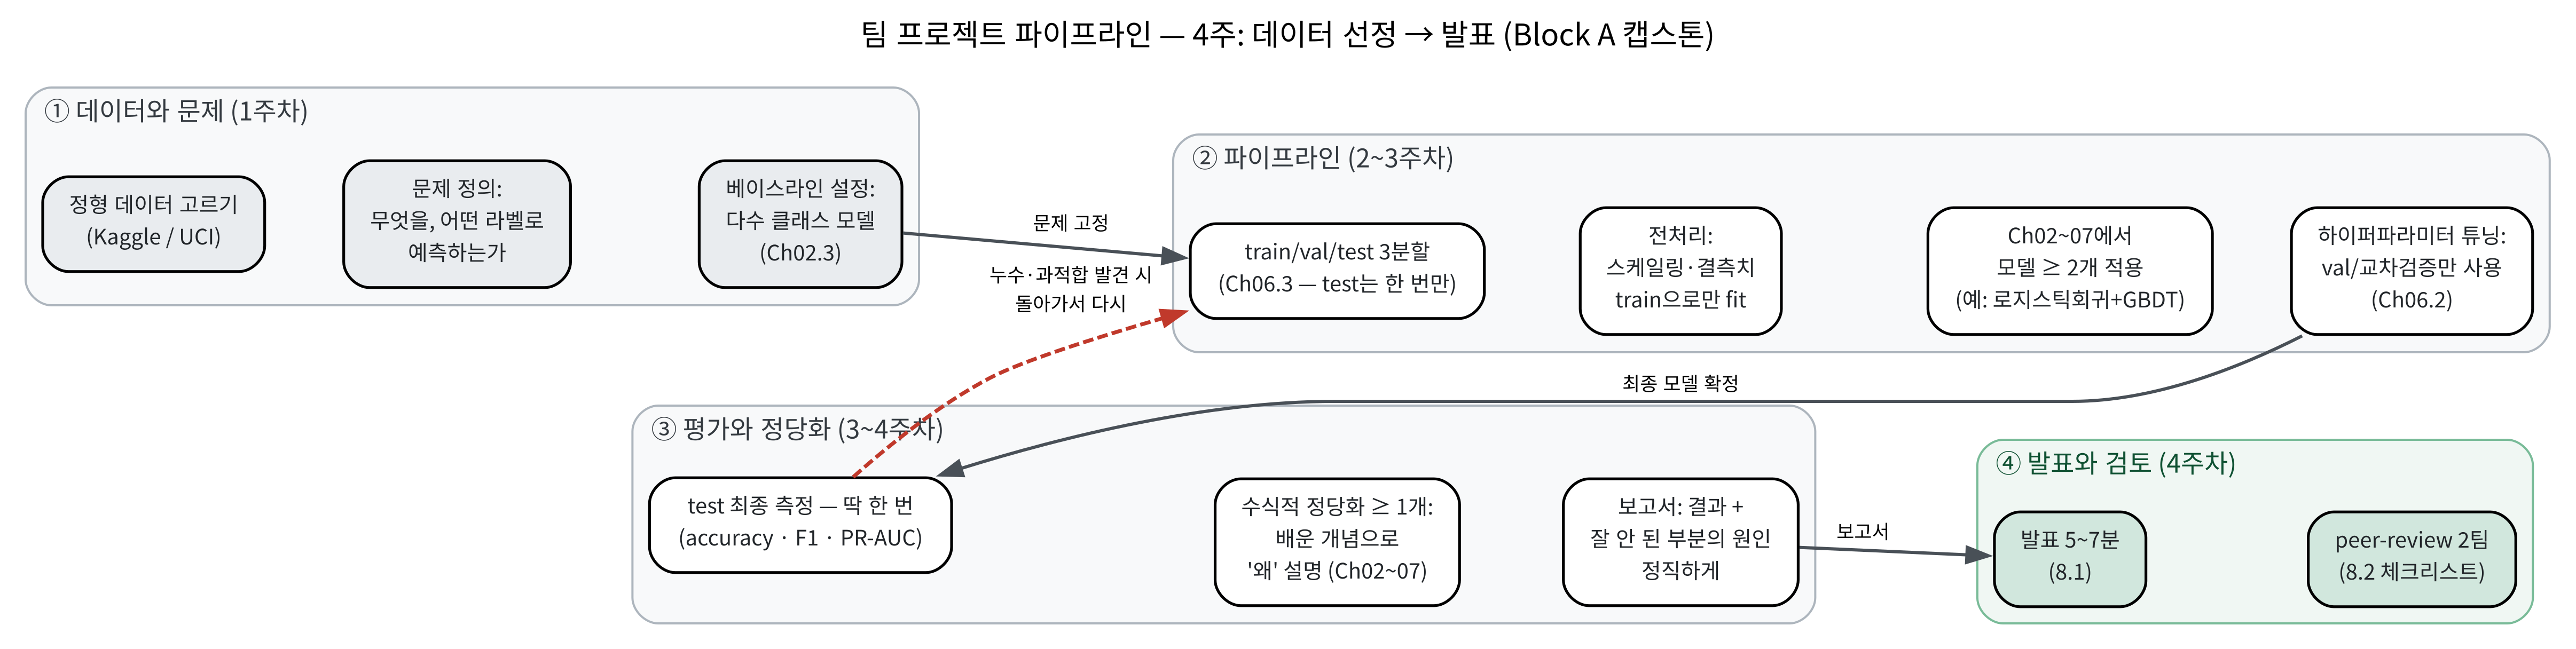
\includegraphics[width=\linewidth]{ch08_1_project_pipeline.png}
      {\footnotesize 데이터·문제 정의(1주) $\to$ 3분할·전처리·
      모델·val 튜닝(2--3주) $\to$ test 한 번·수식적 정당화(3--4주)
      $\to$ 발표·peer-review(4주)}
    \end{column}
    \begin{column}{0.38\textwidth}
      \begin{itemize}
        \item 왼쪽$\to$오른쪽으로 \kb{데이터 $\to$ 파이프라인
          $\to$ 평가 $\to$ 발표} 로 흐름.
        \item \textbf{붉은 점선}이 핵심: test에서 \textbf{누수}
          (Ch.\,6.3)나 \textbf{과적합}(Ch.\,4.1)이 보이면
          돌아가서 다시.
        \item ``한 번 지나가면 돌아올 수 없는 것''은
          \textbf{test 한 번의 측정}뿐 --- 그 외 모든 단계는
          되돌아갈 수 있다.
      \end{itemize}
    \end{column}
  \end{columns}
\end{frame}

\begin{frame}[allowframebreaks]{일정과 마일스톤 M1--M4}
  \small
  \begin{tabular}{@{}clp{7.2cm}@{}}
    \toprule
    주 & 해야 할 일 & 마일스톤(제출) \\
    \midrule
    1 & 데이터 후보 2$\sim$3개 조사(크기·결측치·클래스 비율),
        팀 회의, \textbf{문제 정의 문서}(행이 무엇인지, 라벨,
        주 지표, 베이스라인) & \textbf{M1} 문제 정의 + 데이터
        선택(1p) \\
    2 & 3분할(Ch.\,6.3)로 코드 스캐폴드, train으로만 fit하는
        전처리, 1개 모델 엔드투엔드, 베이스라인 측정 &
        \textbf{M2} 중간코드 리뷰(코드 + 베이스라인 1줄) \\
    3 & 나머지 모델 적용, val/교차검증(Ch.\,6.2)으로 튜닝,
        \textbf{test 최종 측정(한 번만)}, 학습 곡선 도출 &
        \textbf{M3} 학습 곡선 1장 + 최종 test 숫자 \\
    4 & 수식적 정당화 작성, 보고서·슬라이드 완성,
        \textbf{발표(5$\sim$7분)}, \textbf{peer-review 2팀} &
        \textbf{M4} 보고서 + 발표 + 리뷰 2건 \\
    \bottomrule
  \end{tabular}
  \vskip0.6em
  \begin{block}{왜 마일스톤이 이 모양인가}
    M2가 \textbf{베이스라인 숫자 한 줄}을 요하는 이유: 이 숫자를
    봐야 ``모델을 만들었다''고 말할 수 있는지 판정 가능.
    M3가 \textbf{학습 곡선 한 장}을 요하는 이유: 최종 숫자만
    제출하면 하이퍼파라미터를 어떻게 정했는지 검증 못 함 ---
    곡선이 있으면 val 곡선이 실제로 선택에 쓰였는지가
    그림에서 드러남.
  \end{block}
\end{frame}

\begin{frame}{프로젝트 구조}
  \begin{itemize}
    \item \kb{데이터} --- Kaggle, UCI Machine Learning Repository
      \textbf{중에서 정형(행/열) 데이터 하나} --- 이미지·텍스트보다
      표 형태가 Ch.\,2--7 모델 검증에 적합.
    \item \kb{적용} --- Ch.\,2--7 중 \textbf{최소 두 가지 모델}
      (예: 로지스틱회귀 + GBDT)을 같은 데이터에 적용해 비교.
    \item \kb{필수: 수식적 정당화 $\geq$1개} ---
      \begin{enumerate}
        \item 정규화 적용했다면 Ch.\,6 편향-분산 관점에서 왜 성능이
          바뀌었는지,
        \item GBDT 썼다면 Ch.\,7 SHAP으로 예측 하나를 분해,
        \item 모델 여러 개 비교했다면 Ch.\,2.3 PR-AUC로 불균형을
          고려한 비교.
      \end{enumerate}
    \item \kb{검증 원칙} --- Ch.\,6.3의 train/validation/test 3분할
      준수, \textbf{테스트 성능은 딱 한 번}만 확인.
  \end{itemize}
\end{frame}

\begin{frame}{데이터 고르기 실전 가이드 5개}
  후보에 ``점수''를 매겨보면 팀 회의가 쉬워진다:
  \begin{enumerate}
    \item \kb{행의 물리적 단위}를 한 문장으로 설명할 수 있는가
      (환자? 거래? 주문?) --- 설명이 안 되면 ``예측 대상 단위를
      일반화하는가''를 물을 수 없다.
    \item \kb{레이아웃의 함정}이 있는가 --- 같은 환자의 여러 검사
      결과가 여러 행이면 무작위 분할이 누수 $\to$
      \texttt{GroupKFold} 필요.
    \item \kb{시계열은 시간순}으로 나눠야 한다(6.3절 노트북 §5).
    \item \kb{클래스 비율을 먼저 보고 지표를 정한다} --- 99:1이면
      정확도가 아니라 PR-AUC/재현율(Ch.\,2.3 정확도의 함정).
    \item \kb{크기} --- 100행 미만이면 CV 폴드가 너무 작아 숫자가
      극도로 흔들림 $\to$ 500$\sim$10{,}000행이 편함.
  \end{enumerate}
\end{frame}

\begin{frame}{후보 데이터셋 한 줄 점검표}
  \scriptsize
  \begin{tabular}{@{}lcll@{}}
    \toprule
    데이터셋 & 크기 & 문제 정의 & 주의할 함정 \\
    \midrule
    breast\,cancer (UCI) & 569$\times$30, 약 4:6 & 조직이 악성인가
      & 비교적 깨끗함 --- ``기본 코스'' \\
    Heart Failure (UCI) & 1{,}000$\times$14, 약 7:3 & 28일 내 사망
      & 약간 불균형 --- F1·PR-AUC 함께 \\
    Poker Hand (UCI) & 1{,}025$\times$13, 10클래스 & 패 손 등급
      & 다중 클래스 --- 베이스라인 10\%(무작위) \\
    Space Guests (Kaggle) & 4{,}500$\times$14, 균형 & 목적지 성좌
      & 결측치 다수 --- 대체를 \textbf{train으로만} \\
    Credit Card (Kaggle) & 28만$\times$31, 99.8:0.2 & 사기 탐지
      & 극단 불균형 --- 정확도 금지, PR-AUC 필수 \\
    \bottomrule
  \end{tabular}
  \vskip0.8em
  \begin{block}{권장 순서}
    ``기본 코스'' breast\_cancer를 먼저 끝내고, 시간이 남으면
    Credit Card 같은 극단 데이터로 \textbf{지표 선택의 중요성}을
    재확인한다 --- 8.2절에서 ``정확도의 함정''을 근거로 리뷰할
    실력이 된다.
  \end{block}
\end{frame}

\begin{frame}{베이스라인: ``모델보다 먼저 봐야 할 숫자''}
  \begin{columns}[T]
    \begin{column}{0.56\textwidth}
      \begin{block}{다수 클래스(majority-class) 모델}
        모델을 \textbf{아예 안 만들고도} 성능을 만드는 유일한
        방법: train에서 가장 많이 나온 클래스를 전부 예측.
      \end{block}
      \vskip0.4em
      \begin{itemize}
        \item 클래스 비율 50:50 $\to$ 베이스라인 정확도 50\%.
        \item 90:10 $\to$ 90\%, \; 99.8:0.2 $\to$ 99.8\%.
        \item 비율을 보면 베이스라인이 \textbf{자동으로 정해진다}.
      \end{itemize}
    \end{column}
    \begin{column}{0.42\textwidth}
      \kq{``우리 test 정확도가 99.8\%''라는 발표는, 베이스라인을
            보지 않은 한 \textbf{아무것도 말하지 않은} 발표다.}
      \vskip0.8em
      Ch.\,2.3 ``정확도의 함정''을 숫자로 강제하는 체크 ---
      보고서는 모델 성능 숫자와 함께 \textbf{항상 베이스라인
      숫자도 함께} 제시.
    \end{column}
  \end{columns}
\end{frame}

\begin{frame}{손으로 한 번: 베이스라인의 F1}
  8.2절 사기 탐지 데이터(99.8:0.2)에서 다수 클래스(정상)만
  찍으면:
  \begin{itemize}
    \item 부정(fraud)에 대한 정확도는 $P=1.0$ 이지만 \textbf{재현율
      $R=0$} --- 부정 건을 하나도 못 잡음.
    \item \[ F_1 = \frac{2PR}{P+R} = 0 \]
  \end{itemize}
  반대로 부정만 전부 맞히려는 극단(전부를 부정으로 찍기)에서는:
  \begin{itemize}
    \item 재현율은 $R=1.0$ 이지만 정확도는 $0.2\%$ 수준으로 희석.
    \item \[ F_1 \approx 0.004 \]
  \end{itemize}
  \vskip0.4em
  \begin{block}{교훈}
    F1은 정확도보다 이런 \textbf{극단적 모델을 더 가혹하게
    (= 정확하게)} 다뤄준다 --- 바로 이것이 지표를 고르는
    이유다.
  \end{block}
\end{frame}

\begin{frame}{모델 비교의 기준: val에서 정하고, test는 한 번만}
  ``최소 두 모델을 비교한다''의 정확한 절차:
  \begin{enumerate}
    \item 모든 후보 모델을 \textbf{train으로만} fit하고,
      \textbf{val 성능으로 순위} 매기기
      (하이퍼파라미터 포함이면 val 안에 Ch.\,6.2 교차검증 사용).
    \item \textbf{val 순위 1등}을 최종 모델로 결정.
    \item 그 모델 \textbf{만} test에 적용해 최종 숫자를
      \textbf{한 번} 얻는다.
  \end{enumerate}
  \vskip0.5em
  \begin{block}{왜 ``한 번''인가}
    test로 후보 $m$개를 돌려봐서 가장 좋은 것을 고르면, 잡음
    $\sigma$ 기준으로 $\mathbb{E}[\max]$만큼 성능이 \textbf{부풀어
    오른다}(Ch.\,6.3 선택 편향 시뮬레이션). 형식적 원칙이
    아니라 \textbf{정량적} 이유다.
  \end{block}
\end{frame}

\begin{frame}{선택 편향의 크기: 후보 50개면?}
  \begin{columns}[T]
    \begin{column}{0.52\textwidth}
      \textbf{본 프로젝트 규모}: 모델 5개 $\times$ 하이퍼파라미터
      후보 10개 $=$ \textbf{후보 50개}. 잡음 $\sigma=0.02$
      (F1 스케일)로 가정하면 부풀림 약 \textbf{0.045}.
      \vskip0.6em
      \kq{``test F1 0.97''이 실제로는 0.925일 수 있다는
      뜻이다.}
      \vskip0.6em
      \begin{itemize}
        \item val로 고르면 \textbf{val이} 이 편향을 먹고,
          test는 한 번만 쓰이므로 부풀림이 test에 \textbf{전이
          되지 않는다}.
        \item 3분할 원칙은 ``정직한 test 숫자''를 사기 위한
          \textbf{구조}.
      \end{itemize}
    \end{column}
    \begin{column}{0.46\textwidth}
      \centering
      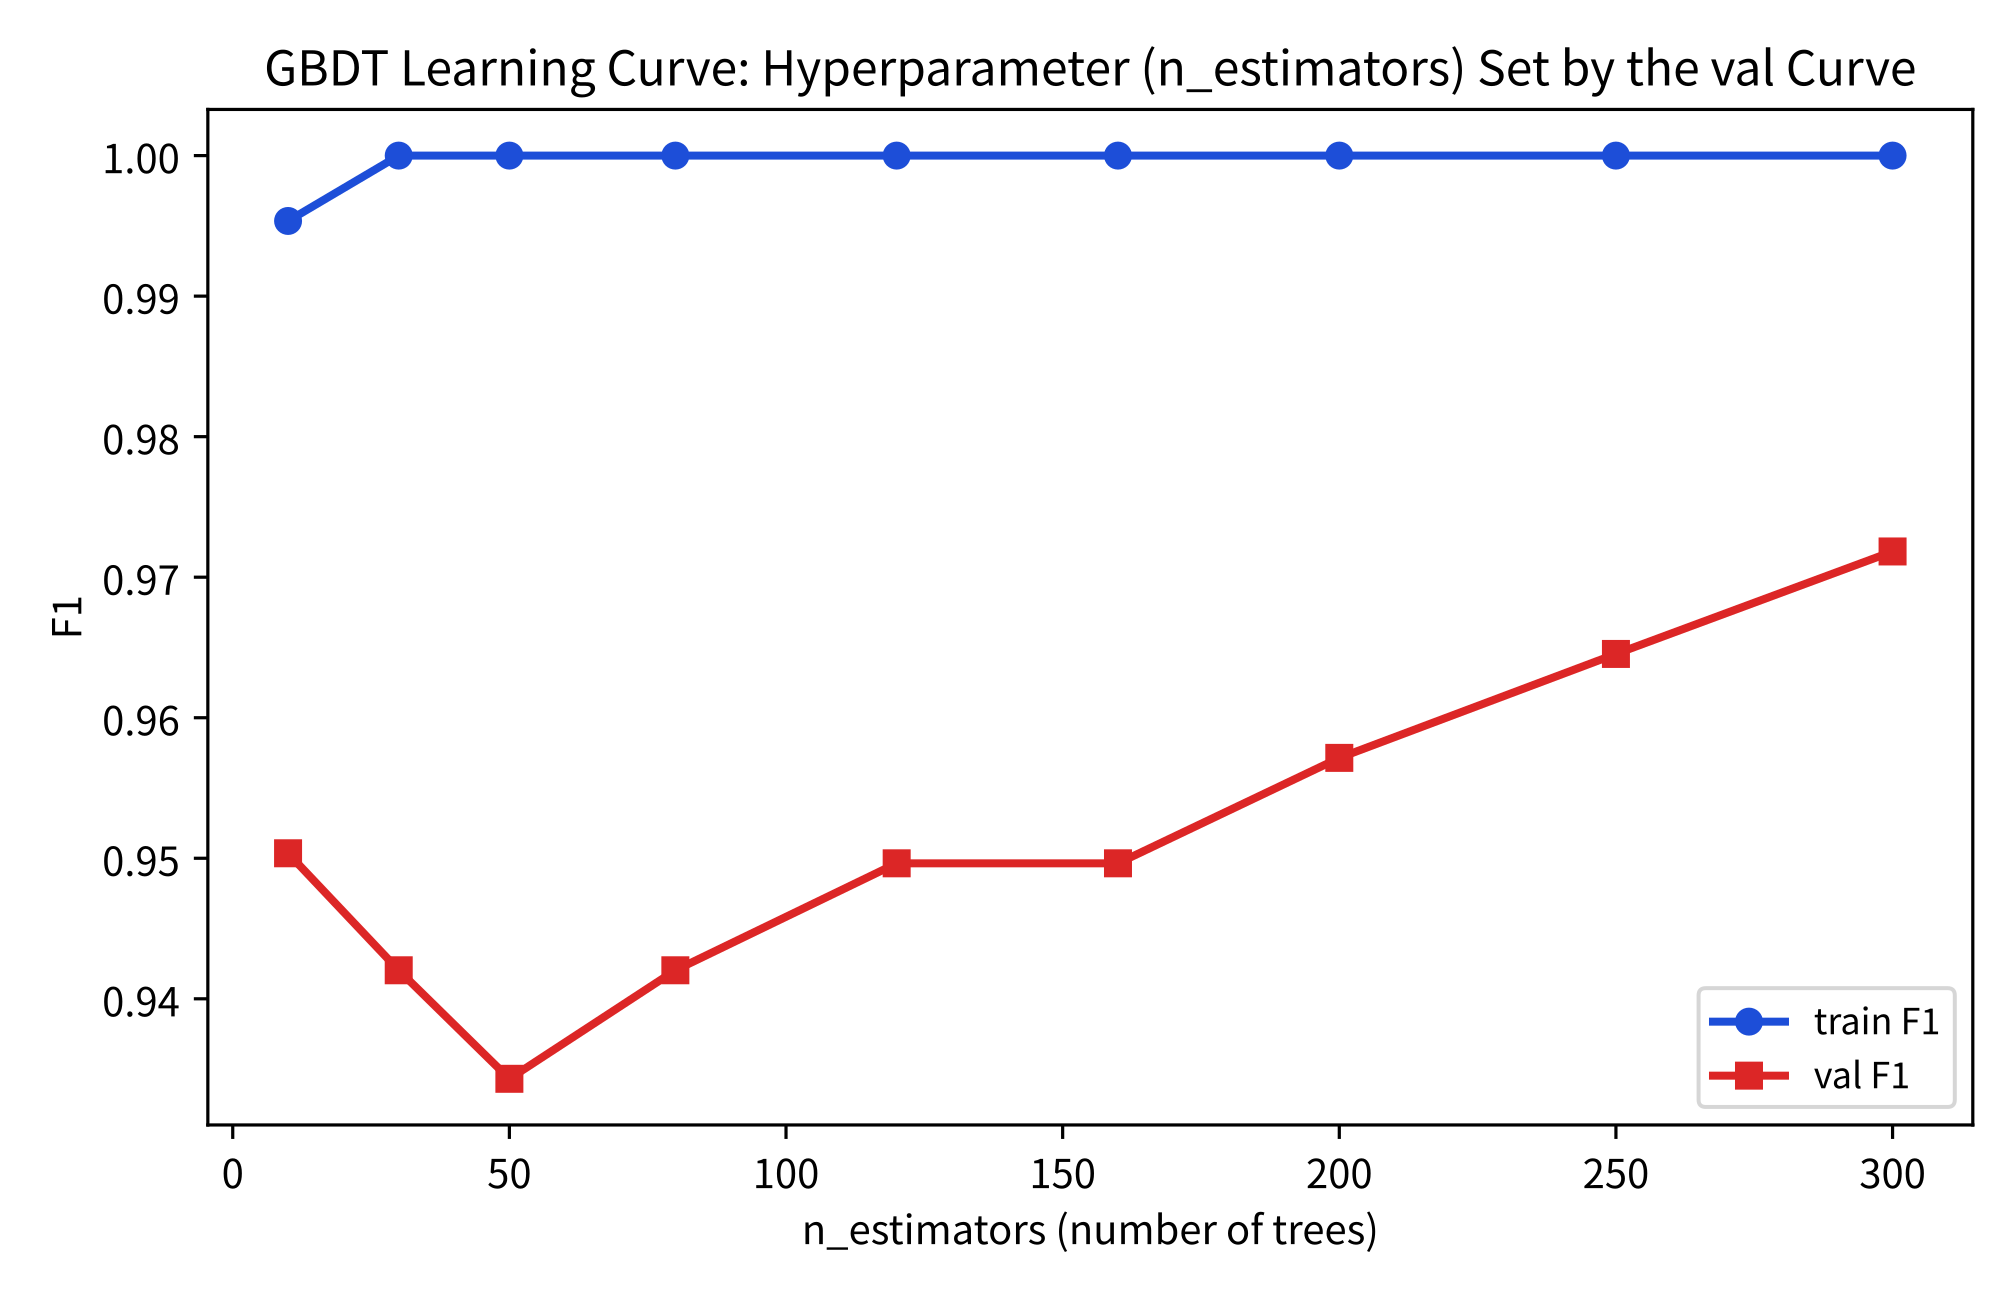
\includegraphics[width=0.98\linewidth]{ch08_1_learning_curve.png}
      {\footnotesize GBDT 학습 곡선 --- train F1은 10개 트리부터
      거의 1.0(341건을 몇 그루면 외우기 쉬움), val F1은
      0.93$\sim$0.97 사이로 느리게 이동. $n_{\text{estimators}}$는
      \textbf{val 곡선으로만} 정한다.}
    \end{column}
  \end{columns}
  \vskip0.3em
  {\footnotesize 6.3절 원칙이 그림에서 바로 보인다: \textbf{train
  곡선은 ``배운 것을'' 재고, val 곡선만 ``재는 것을'' 한다.}
\end{frame}

\begin{frame}{실습: breast\_cancer 한 흐름 9단계}
  \scriptsize
  \begin{tabular}{@{}cl@{}}
    \toprule
    단계 & 내용(실측) \\
    \midrule
    1 & 문제 정의 --- 행=환자, 라벨=양성/악성, 주 지표 F1 \\
    2 & 3분할: train 341 / val 114 / test 114 (stratify,
       unique id로 pairwise disjoint 기계 점검) \\
    3 & 전처리: \texttt{StandardScaler}를 \textbf{train으로만 fit} \\
    4 & 모델 5개 후보(로지스틱·kNN·트리·RF·GBDT) val F1 비교
       $\to$ \textbf{kNN(k=5)가 0.973로 1위} \\
    5 & 베이스라인: 다수 클래스의 val F1 0.774 --- kNN이
       0.198 상회해야 ``모델을 만들었다''고 말할 수 있음 \\
    6 & test 한 번: accuracy 0.939, F1 0.950, PR-AUC 0.979 \\
    7 & 선택 편향 시뮬레이션: test로 5개 후보 고르면 $+0.023$,
       50개면 $+0.045$ 부풀림 \\
    8 & 학습 곡선: GBDT $n_{\text{estimators}}$ vs train/val F1 \\
    9 & SHAP 가산성 2-특징 장난감 손계산:
       $0.50+0.08+0.20=0.78=f(\{A,B\})$ \\
    \bottomrule
  \end{tabular}
  \vskip0.6em
  이 9단계가 곧 \textbf{보고서 6절} $\to$ \textbf{8.2 체크리스트
  4항목}으로 매핑된다 --- 같은 절차를 코드·보고서·리뷰
  \textbf{세 가지 언어}로 말할 수 있어야 프로젝트가 끝난다.
\end{frame}

\begin{frame}{보고서 구조 (M4) --- 발표 슬라이드 = 보고서의 각 절 제목}
  \small
  \begin{tabular}{@{}llp{7.6cm}@{}}
    \toprule
    절 & 분량 & 내용 \\
    \midrule
    1. 문제 정의 & 0.5p & 행의 단위·라벨·주 지표·베이스라인
       + ``왜 이 지표를 골랐는가'' 한 문장 \\
    2. 데이터와 전처리 & 1p & 원본 통계(크기·결측치·이상치),
       \textbf{train으로만 fit한 전처리} 명시, 3분할 비율 +
       stratify 여부 \\
    3. 모델 선택과 이유 & 1$\sim$2p & 후보 $\geq$2개, \textbf{왜
       이 후보들인가} (데이터 특성과 연결: 거리 기반이면
       스케일링, 트리 기반이면 불필요), val 비교 표 \\
    4. 결과 & 1p & 최종 test 숫자(한 번), 학습 곡선 1장, val 표 \\
    5. 수식적 정당화 & 1p & 편향-분산·정규화·SHAP·PR-AUC 중
       $\geq$1개로 ``왜 이 결과가 나왔는지'' \\
    6. 잘 안 된 부분과 원인 진단 & 0.5p & \textbf{필수} --- 없었으면
       ``무엇을 시도했다가 안 됐는가''. 이 절이 비어 있으면
       ``결과의 정직성'' 항목을 의심받음 \\
    \bottomrule
  \end{tabular}
\end{frame}

\begin{frame}{채점 기준 (rubric)}
  \small
  \begin{tabular}{@{}lcl@{}}
    \toprule
    항목 & 비중 & 좋은 답 \\
    \midrule
    문제 정의와 데이터 & 15\% & 행의 단위·라벨·지표·베이스라인
       명확, 지표 선택이 데이터 특성에 근거 \\
    방법론 적절성 & 25\% & 데이터 특성(불균형·차원·시계열·그룹)에
       맞는 모델·전처리·분할, Ch.\,2--7 개념으로 근거 \\
    검증의 정직성 & 25\% & 3분할·train-fit·test 한 번·베이스라인
       ·학습 곡선·val 튜닝이 \textbf{추적 가능}할 정도로 명시 \\
    수식적 정당화 & 20\% & 개념 $\geq$1개로 ``왜'' 설명 + 설명이
       관측(숫자)과 일치 \\
    결과의 정직성과 반성 & 15\% & 잘 안 된 부분을 숨기지 않고
       Ch.\,2--7 개념으로 원인 진단 \\
    \bottomrule
  \end{tabular}
  \vskip0.7em
  \begin{block}{50\%가 절차인 이유}
    목적이 ``높은 성능''이 아니라 \textbf{``성능 숫자를 정직하게
    얻는 절차''를 수행한 것을 증명}하는 것이기 때문. 성능 0.60
    이어도 절차가 정직하면 높은 점수, 0.99여도 test를 두 번 썼거나
    베이스라인이 없으면 크게 감점.
  \end{block}
\end{frame}

\begin{frame}{수식적 정당화: 나쁜 설명 vs 좋은 설명}
  같은 결과(``정규화 적용 $\to$ test 정확도 0.89$\to$0.93'')를
  설명하는 두 문장:
  \begin{columns}[T]
    \begin{column}{0.48\textwidth}
      \begin{alertblock}{나쁜 설명}
        ``정규화를 넣으니까 성능이 좋아졌다. 정규화가 좋은
        방법인 것 같다.''
      \end{alertblock}
      \vskip0.5em
      {\footnotesize 관찰만 있고 \textbf{왜}가 없다.}
    \end{column}
    \begin{column}{0.48\textwidth}
      \begin{block}{좋은 설명}
        정규화 없이 train 0.99 / test 0.89 --- 큰 격차(Ch.\,4.1
        의 분산 큰 과적합). L2 추가 + Ch.\,6.2 교차검증으로
        $\lambda$ 튜닝 $\to$ train 0.95로 약간 하락, test 0.93
        으로 상승 --- \textbf{train/test 격차가 줄어든 것}이
        정규화가 실제로 분산을 줄인 증거.
      \end{block}
    \end{column}
  \end{columns}
  \vskip0.5em
  \kq{``성능이 올랐다''는 관찰과 ``왜 올랐는지 설명할 수
  있다''는 이해는 다른 수준의 성취다.}
\end{frame}

\begin{frame}{``살짝 훔쳐보기''가 얼마나 성능을 부풀리는가}
  각 후보의 test 성능을 (진짜 성능 + 잡음
  $\mathcal{N}(0,\sigma^2)$)으로 모델링하면, 후보 $m$개 중
  \textbf{최고 점}을 고르는 것은 $m$번 잡음 뽑기의 max ---
  항상 낙관 쪽으로 치우친다.
  \vskip0.5em
  \small
  \begin{tabular}{@{}ll@{}}
    \toprule
    후보 수 $m$ & $\mathbb{E}[\max]$ (부풀림) \\
    \midrule
    1 (test 안 쓰고 val로만 고른 경우) & $\approx 0$ \\
    5 (모델 5개만 test로 비교) & $\approx 0.023$ \\
    50 (5개 모델 $\times$ 하이퍼파라미터 10개) & $\approx 0.045$ \\
    100 & $\approx 0.050$ \\
    \bottomrule
  \end{tabular}
  \vskip0.6em
  \begin{block}{읽는 법}
    ``5개 모델을 test로 돌려보고 제일 좋은 것을 골랐다''는
    행위는 F1 0.97의 결과에 \textbf{실제로 0.947일 수 있다}는
    불확실성을 안고 있다. 후보가 \textbf{모델 수 $\times$
    하이퍼파라미터 수}의 곱으로 커지는 것이 이 편향이
    4.5\%p가 되는 이유.
  \end{block}
\end{frame}

\begin{frame}{자주 하는 실수 5가지}
  각각이 Ch.\,2--7의 어떤 원칙을 깨는지 짚어두면, 8.2절에서
  바로 반박 가능한 질문으로 바꿀 수 있다:
  \begin{enumerate}
    \item \kb{테스트로 모델 고르기} (``살짝 훔쳐보기'') --- 선택
      편향을 test에 그대로 전이. \textit{리뷰 질문}: ``val F1
      순위와 test F1 순위가 같은가요? 시드 3개로 확인할 수
      있나요?''
    \item \kb{정규화/결측치 통계를 전체 데이터로 fit} --- 6.3절의
      ``정규화 통계량 누수''. \texttt{fit(X\_train)} $\to$
      \texttt{transform(X\_val)}, \texttt{transform(X\_test)}
      가 정석.
    \item \kb{베이스라인 없이 성능 보고} --- 클래스 비율 90:10에서
      ``정확도 91\%''는 아무것도 말하지 않는다.
    \item \kb{시계열/그룹 데이터의 무작위 분할} --- ``비현실적으로
      좋은'' 성능, \textbf{배포(새 환자/미래 시간)에서는 완전히
      붕괴}.
    \item \kb{학습 곡선 없이 하이퍼파라미터 보고} --- ``lr=0.1을
      썼다''가 왜 0.05·0.3이 아니라 0.1인지 val 곡선 없이는
      확인 불가(M3가 학습 곡선을 요구하는 이유).
  \end{enumerate}
\end{frame}

\begin{frame}{발표: 5$\sim$7분의 설계도}
  \begin{center}
    \small
    \begin{tabular}{@{}lcl@{}}
      \toprule
      순서 & 내용 & 시간 \\
      \midrule
      1 & 문제 정의 & 1분 \\
      2 & 데이터와 전처리 & 1분 \\
      3 & 적용한 모델과 이유 & 2분 \\
      4 & 결과와 수식적 정당화 & 2분 \\
      5 & 잘 안 됐던 부분과 원인 진단 & 1분 \\
      \bottomrule
    \end{tabular}
  \end{center}
  \vskip0.5em
  \begin{itemize}
    \item ``정확도 90\% 달성''보다 \textbf{``왜 이 모델을 골랐고
      왜 이 결과가 나왔는지''}를 설명하는 쪽에 높은 점수.
    \item 마지막 1분(``잘 안 됐던 부분'')이 \textbf{가장
      평가받는} 부분 --- rubric의 ``결과의 정직성과 반성''이
      정확히 여기 를 본다.
    \item ``모든 것이 잘 됐다''는 발표는 이 항목에서 \textbf{스스로
      감점}. ML2의 Ch.\,16.1(강화학습 캡스톤)도 동일한 구조.
  \end{itemize}
\end{frame}

\begin{frame}{발표의 마지막 1분: 실패를 개념으로 해석하라}
  \begin{columns}[T]
    \begin{column}{0.48\textwidth}
      \begin{alertblock}{``모든 것이 잘 됐다''}
        ``결과의 정직성과 반성'' 항목에서 \textbf{스스로 감점}을
        받는 발표 --- 이 절이 비어 있다는 뜻.
      \end{alertblock}
    \end{column}
    \begin{column}{0.48\textwidth}
      \begin{block}{점수받는 발표}
        ``트리 깊이를 5로 늘리자 val F1이 0.97에서 0.95로
        떨어졌다 --- Ch.\,7.3대로 GBDT가 잔차를 계속 쫓다
        노이즈까지 학습하기 시작한 것으로 진단하고, 깊이를
        3으로 고정했다.''
      \end{block}
    \end{column}
  \end{columns}
  \vskip0.5em
  \begin{itemize}
    \item 실패한 시도를 \textbf{배운 개념으로 해석한} 증거라서
      더 높은 점수.
    \item ``시간 부족으로 3번째 모델을 못 돌렸다''를 \textbf{정직하게
      쓰는 것}이 성능 숫자를 부풀리는 것보다 항상 낫다.
  \end{itemize}
\end{frame}

\begin{frame}{확인 문제 (1)}
  \begin{itemize}
    \item \textbf{1.} 팀이 train 70\% / test 30\%만 쓰고
      하이퍼파라미터를 \textbf{test로} 고르겠다고 한다. 후보 10개,
      잡음 $\sigma=0.01$일 때 test 성능이 평균적으로 얼마나
      부풀어 오르는가?
      \vskip0.3em
      {\footnotesize \textbf{답}: Ch.\,6.3 $\mathbb{E}[\max]$ 계산
      ($\sigma=1$일 때 $\approx 1.53$)에 $\sigma=0.01$을 곱하면
      $\approx 0.015$ --- test F1이 실제로 0.985인데 1.00으로
      보고될 수 있다. 질문 예: ``시드 5개로 val/test 순위의
      불일치율을 재볼 수 있나요?''}
    \item \textbf{2.} breast\_cancer(악성 62.7\%)에서 다수 클래스
      베이스라인의 val F1은 0.774였다. \textbf{정확도} 지표의
      베이스라인은? 왜 정확도가 F1보다 ``인정하기 쉬운''
      숫자인가?
      \vskip0.3em
      {\footnotesize \textbf{답}: 정확도 베이스라인 $\approx$ 62.7\%.
      정확도는 소수 클래스 몇 건을 잡았는지를 \textbf{희석}한다
      --- 50:50이 아니면 모델과 베이스라인의 차이를 과소/과대
      평가. F1은 희석 효과를 없애므로 적합.}
  \end{itemize}
\end{frame}

\begin{frame}{확인 문제 (2)}
  \begin{itemize}
    \item \textbf{3.} 같은 데이터를 (a) 무작위 분할, (b)
      환자(그룹) 분할로 나눠 kNN을 학습하면 (a)의 test RMSE가
      비현실적으로 낮아진다. (a)가 왜 좋은 성적을 내는가?
      \vskip0.3em
      {\footnotesize \textbf{답}: (a)에서는 같은 환자의 여러 행이
      train/test에 흩어져, kNN이 test 행의 k-이웃을 \textbf{같은
      환자의 train 행}으로 찾아 ``환자를 인식''한다 --- 관계를
      배운 것이 아니라 환자를 \textbf{외운} 것. 질문: ``그룹 키
      (환자 ID)가 있는가? \texttt{GroupKFold}로 재분할하면?''}
    \item \textbf{4.} ``GBDT $n_{\text{estimators}}$=300을 val
      곡선으로 정했다''는데, val F1이 300에서 \textbf{계속
      상승 중}이다. 한계는?
      \vskip0.3em
      {\footnotesize \textbf{답}: 상승 중이면 ``300이 최적''이
      아니라 ``관찰 범위 내 최선''. val이 $n\approx150$에서 정점
      후 하락했다면 300은 train F1=1.0 포화 상태에서 \textbf{잔차
      (노이즈)를 쫓다 overfit한} 구간 --- 150 부근(early
      stopping)을 골랐어야 함. 기준은 언제나 \textbf{val 정점}.}
  \end{itemize}
\end{frame}

\begin{frame}{자주 묻는 질문}
  \begin{itemize}
    \item \textbf{Q. 두 모델 성능이 거의 같으면?} 오히려 좋은 소재
      --- Ch.\,6.3: 차이가 검증셋 표본 크기에 비해 작다면
      ``우연''일 수도 있다는 것 자체가 \textbf{통계적으로 중요한
      관찰}. 예측이 어떤 포인트에서 갈리는지, 어느 쪽이 해석하기
      쉬운지(로지스틱의 계수 vs GBDT의 SHAP)로 채운다.
    \item \textbf{Q. 결측치·이상치가 많은 데이터는 감점?} 아니다
      --- 오히려 전처리 결정(어떻게 채웠는지, 이상치를 제거·유지
      했는지)과 \textbf{그 근거}가 좋은 평가 포인트. ``지저분한
      데이터를 다룬 판단 과정''이 실전에 훨씬 가깝다.
    \item \textbf{Q. 역할 분담은?} 데이터·코드·보고서·발표를
      \textbf{팀 전체가 함께 결정}하되 작성은 나눠도 된다.
      ``코드는 A, 보고서는 B''로 완전히 분리하면 B가 A의 코드를
      모르는 채 정당화를 쓰게 됨(=``나쁜 설명'') --- M2
      중간코드 리뷰가 이를 강제.
    \item \textbf{Q. 4주 안에 안 끝날 것 같은데?} 성공 기준은
      ``높은 성능''이 아니라 \textbf{``정직한 절차''} --- 모델을
      2개로 줄이고(최소선은 2개) ``시간 부족으로 3번째 모델을
      못 돌렸다''를 정직하게 쓰는 것이 부풀리기보다 낫다.
  \end{itemize}
\end{frame}

\section{8.2 Peer-Review}

\begin{frame}{역전: 이번엔 네가 심사위원이다}
  \begin{itemize}
    \item 8.1에서 각 팀이 발표를 마쳤다면, 8.2에서는
      \textbf{역전} --- 다른 \textbf{두 팀}의 발표를 듣고,
      체크리스트로 리뷰를 쓰고, \textbf{리뷰의 품질로 네가
      채점}받는다.
    \item ML 결과는 \textbf{잘못된 것이 아니라 우연히 좋은 것처럼
      보이는 것}이 너무나 쉽다:
      \begin{itemize}
        \item test를 하이퍼파라미터 튜닝에 써서 (Ch.\,6.3 선택
          편향),
        \item 클래스가 99.8:0.2로 기울어 있어서 (Ch.\,2.3 정확도
          의 함정),
        \item train에 과적합해서 (Ch.\,6.1).
      \end{itemize}
  \end{itemize}
  \vskip0.4em
  \begin{block}{그러므로}
    ``좋은 결과''는 \textbf{스스로를 증명하지 못한다} ---
    다른 누군가가 그 결과를 \textbf{뒤집을 수 있는 구체적인
    방법}을 찾아내는지로 판단해야 한다.
  \end{block}
\end{frame}

\begin{frame}{Popper의 반증주의: 왜 ``반박 가능''인가}
  \begin{columns}[T]
    \begin{column}{0.55\textwidth}
      Karl Popper, 1934년 \textit{The Logic of Scientific
      Discovery}:
      \begin{block}{반증주의 (falsifiability)}
        한 주장은 ``그것이 틀렸음을 보여주는 관측이
        \textbf{원칙적으로} 상상이 가능한가''로 판별된다.
        \textbf{반박될 수 없는 주장은 과학이 아니다.}
      \end{block}
    \end{column}
    \begin{column}{0.43\textwidth}
      \kb{peer-review의 적용}
      좋은 질문이란 \textbf{발표팀이 제대로 답하지 못하면
      결과 자체가 흔들리는} 질문:
      \begin{itemize}
        \item ``더 잘 설명해 주세요'' = \textbf{요청}.
        \item ``Ch.\,6 교차검증 없이 $\lambda$를 정했는데, 그
          검증 성능이 우연일 가능성은 없는가?'' = \textbf{반박}.
      \end{itemize}
    \end{column}
  \end{columns}
\end{frame}

\begin{frame}{Amgen 재현 실험 (2011)}
  \begin{columns}[T]
    \begin{column}{0.55\textwidth}
      \begin{itemize}
        \item 생물제약 회사 Amgen이 1999$\sim$2005년 발표된
          ``주요(landmark)'' 생물학 논문 \textbf{53편}을 직접
          재현하려 했다.
        \item \textbf{6편밖에} 재현되지 못했다.
        \item 47편은 ``잘못되었다기보다 재현이 안 된다'' ---
          이후 \kb{재현성 위기} 논쟁의 상징이 되었다.
      \end{itemize}
    \end{column}
    \begin{column}{0.43\textwidth}
      \begin{block}{peer-review의 정체}
        ``남의 발표를 까탈스럽게 까는 절차''가 \textbf{아니다}
        --- Amgen이 스스로 했던 것과 동일한 행위:
        \textbf{내 결과도 남이 재현·반박할 수 있도록 미리
        방어하는 것}.
      \end{block}
      \vskip0.4em
      \kq{네 발표 전에, 네가 심사할 때 던질 가장 날카로운
           질문을 스스로 던져 답을 준비해 두는 것이 최선.}
    \end{column}
  \end{columns}
\end{frame}

\begin{frame}{이번 주 진행: 세 단계 + 체크리스트}
  \small
  \begin{tabular}{@{}clp{6.4cm}@{}}
    \toprule
    순서 & 내용 & 시간 \\
    \midrule
    1 & 다른 두 팀 발표 청취(각 5$\sim$7분, 8.1 형식) &
      50분 중 약 30분 \\
    2 & 체크리스트 기반 \textbf{작성 리뷰 두 통} --- 팀당 4개
       항목 + \textbf{반박 가능한 질문 1개 이상} & 발표 직후 \\
    3 & 질의·토론: 리뷰어가 쓴 질문에 발표팀이 답변 &
      나머지 시간 \\
    \bottomrule
  \end{tabular}
  \vskip0.5em
  \begin{tabular}{@{}lp{10.2cm}@{}}
    \toprule
    체크리스트 4항목 & 확인할 것 \\
    \midrule
    \kb{문제 정의} & 무엇을 예측/분류하려 했는지 명확한가 \\
    \kb{방법론 적절성} & 데이터 특성(불균형, 차원 수 등)에 맞는
      모델을 골랐는가 \\
    \kb{수식적 정당화} & 요구사항을 충족했고, 그 설명이 실제로
      타당한가 \\
    \kb{결과의 정직성} & 잘 안 된 부분을 숨기지 않고 원인을
      분석했는가 \\
    \bottomrule
  \end{tabular}
  \vskip0.4em
  {\footnotesize 8.1에서 ``수식적 정당화''가 발표팀의 \textit{의무}였다면,
  이번 주는 그 정당화가 \textit{타당한지}를 \textbf{리뷰어가
  심사}한다.}
\end{frame}

\begin{frame}{채점 기준: ``채웠는가''가 아니라 ``구체적인가''}
  \small
  \begin{tabular}{@{}llp{7.8cm}@{}}
    \toprule
    품질 & 특징 & 예시 \\
    \midrule
    1점 --- 감상평 & 구체적 지적이 없음, 느낌만 &
      ``발표 잘 들었습니다. 결과가 인상적이네요.'' \\
    2점 --- 일반 지적 & 문제를 제기하지만 \textbf{근거(개념)가
      약함} --- 발표팀이 ``네''로 넘길 수 있음 &
      ``모델 선정 이유가 부족해 보입니다. 데이터 특성을 더
      봐주세요.'' \\
    3점 --- 반박 가능 & \textbf{장·절을 명시}하고, 답이 나쁘면
      결과가 흔들리는 질문 & ``불균형(99.8:0.2)에 정확도만
      비교했는데(Ch02.3), Precision·Recall을 안 주면 '둘 다
      항상 정상으로 찍는' 모델일 수 있는데 어떻게 구분
      하셨나요?'' \\
    \bottomrule
  \end{tabular}
\end{frame}

\begin{frame}{1점 $\to$ 3점: 공통 패턴}
  \begin{itemize}
    \item 1점$\to$2점$\to$3점으로 올라가는 방향을 보면 공통
      패턴이 하나 --- \textbf{추상적 평가어(``부족하다'',
      ``인상적이다'')를 구체적 관찰 + 이 학기 개념(Ch NN)으로
      교체}하는 것.
    \item ``모델 선정이 부족하다''(2점): 관찰도 개념도
      \textbf{없음}.
    \item ``99.8:0.2 불균형에서 정확도만 비교했다(Ch02.3의
      정확도의 함정)''(3점):
      \begin{itemize}
        \item \kb{관찰} --- 정확도만 쓰셨다,
        \item \kb{개념} --- Ch02.3 정확도의 함정,
        \item \kb{왜 문제인지} --- 항상 정상으로 찍으면 정확도
          99.8\%.
      \end{itemize}
  \end{itemize}
  \vskip0.5em
  \begin{block}{3점 질문의 구조}
    \kq{관찰 + 개념(장·절) + ``왜 문제인지'' --- 세 칸 모두
    채워져야 반박 가능.}
  \end{block}
\end{frame}

\begin{frame}{손으로 한 번: 가상 발표에 체크리스트를 적용}
  \begin{alertblock}{가상 발표 요약}
    ``신용카드 이상거래 데이터로 사기 탐지. 99.8\% 정상, 0.2\%
    사기. 로지스틱회귀 $\to$ 정확도 \textbf{99.7\%}. GBDT $\to$
    \textbf{99.8\%}로 더 높았다. 그래서 GBDT가 더 좋은 모델.``
  \end{alertblock}
  \small
  \begin{tabular}{@{}ll@{}}
    \toprule
    항목 & 판정 \\
    \midrule
    문제 정의 & \checkmark 명확 --- 이상거래 탐지, 이진 분류 \\
    방법론 적절성 & $\times$ 99.8:0.2 극단 불균형에 \textbf{정확도}를
      썼다 --- ``정확도의 함정''(Ch.\,2.3). 99.7 vs 99.8의 차이가
      사기를 더 잘 잡아서인지, \textbf{둘 다 거의 항상 정상}인
      모델인지 구분 안 됨 \\
    수식적 정당화 & $\times$ 형식적으로만 충족 --- 불균형에 맞는
      지표(PR-AUC, 재현율)를 전혀 안 씀 \\
    결과의 정직성 & $\times$ ``GBDT가 더 좋다''는 결론의 근거가
      위 문제 때문에 약함 \\
    \bottomrule
  \end{tabular}
  \vskip0.4em
  {\footnotesize \kb{반박 가능한 질문}: ``두 모델의 Precision과
  Recall을 각각 따로 보여줄 수 있나요?'' --- 막연한 ``더 잘
  설명해 주세요''가 아니라 \textbf{Ch.\,2.3의 구체적 개념}(클래스
  불균형과 정확도의 함정)을 근거로 무엇이 부족한지 짚는다.}
\end{frame}

\begin{frame}{실습: ``정확도 99.8\%''를 코드로 검증 (1)}
  \begin{columns}[T]
    \begin{column}{0.56\textwidth}
      \begin{itemize}
        \item 노트북은 발표의 설정(거래 10만 건, 사기 200건 =
          0.2\%)을 1차원 장난감 데이터로 재현하고, 임계값
          분류자로 정확도·재현율·PR-AUC를 직접 계산.
        \item \kb{(1)} \textbf{``쓸모있는 모델''의 정확도는
          ``무조건 정상''보다 낮다}: 사기를 약 90\% 잡는
          분류자(임계값 $t=2.5$)의 정확도는 \textbf{99.37\%}
          --- 아무 모델 없이 전부 ``정상''을 찍으면
          \textbf{99.8\%}(사기 1건도 못 잡는데도 정확도만으로는
          더 낫다).
      \end{itemize}
      \vskip0.3em
      \kq{정확도 99.8\%가 ``모델이 좋다''는 증거가 아님을
      보여주는 가장 직접적인 숫자.}
    \end{column}
    \begin{column}{0.42\textwidth}
      \centering
      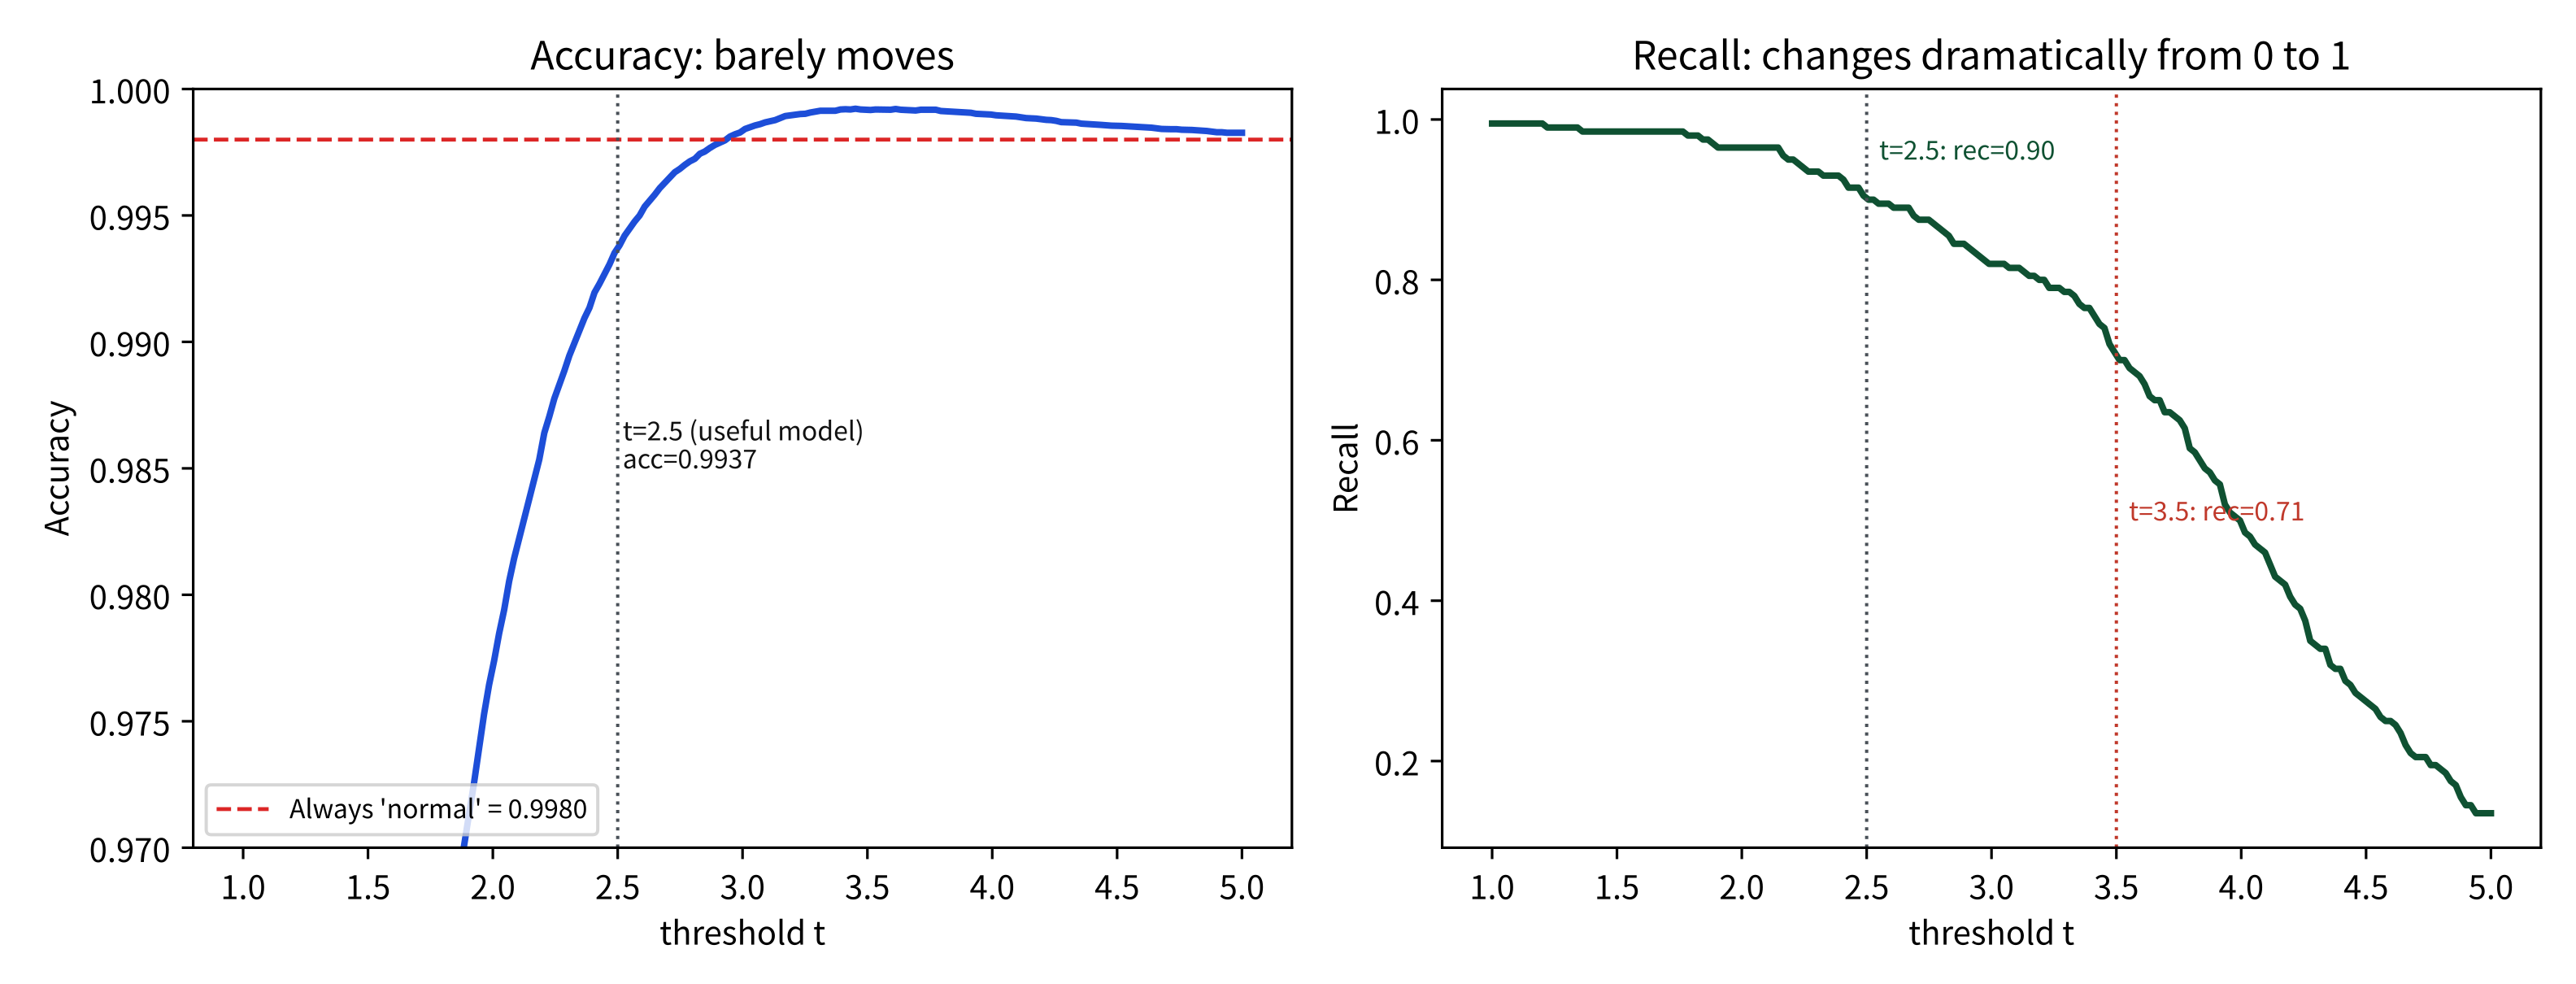
\includegraphics[width=\linewidth]{ch08_2_accuracy_trap.png}
      {\footnotesize 왼쪽: 임계값 $t$ 1.0$\to$5.0을 올리면 정확도는
      99.8\%(무조건 정상, 붉은 점선) 부근에서 거의 움직임이
      없음. 오른쪽: 같은 범위에서 재현율은 0에서 0.99까지
      크게 변한다 --- 정확도로 ``동점''인 동안, 사기를 잡는
      능력은 완전히 다름.}
    \end{column}
  \end{columns}
\end{frame}

\begin{frame}{실습: 정확도 순위와 사기 잡기 순위 (2)}
  같은 분류자에서 \textbf{임계값만} 바꿔도 정반대의 줄 서기:
  \vskip0.4em
  \small
  \begin{center}
  \begin{tabular}{@{}lcccc@{}}
    \toprule
    임계값 $t$ & 정확도 & Precision & 재현율 & F1 \\
    \midrule
    3.5 & \textbf{99.92\%} & 86.1\% & 71.0\% & 77.8\% \\
    2.5 & 99.37\% & 22.8\% & 90.0\% & 36.3\% \\
    2.0 & 97.72\% & 7.8\% & \textbf{96.5\%} & 14.5\% \\
    \bottomrule
  \end{tabular}
  \end{center}
  \vskip0.3em
  \begin{itemize}
    \item 정확도로 줄 세우면 $t=3.5$가 최고, $t=2.0$이 최하.
    \item 사기를 실제로 잡는 능력(재현율)으로는 \textbf{순서가
      완전히 뒤집힌다} ($t=2.0$이 최고).
  \end{itemize}
  \vskip0.3em
  \begin{block}{교훈}
    ``정확도가 높을수록 좋은 모델''이라는 직관이 불균형
    데이터에서는 \textbf{모든 것을 더 놓치는 방식을 최고로
    뽑는} 잘못된 기준이 된다.
  \end{block}
\end{frame}

\begin{frame}{실습: 동점의 함정 (3) --- 의미를 가진 지표는 PR-AUC}
  \begin{itemize}
    \item 발표 설정(로지스틱회귀 vs GBDT)을 실제 2차원 불균형
      데이터로 재현하면: test 정확도는 \textbf{99.86\% vs
      99.80\%} --- 0.06\%p 차이, \textbf{검증셋 잡음보다 작거나
      같은} 크기.
    \item 그런데 PR-AUC는 \textbf{0.636 vs 0.071}로 확연히
      달라진다 --- 정확도 하나만 보면 ``둘이 같다'', PR-AUC를
      보자니 차이는 컸다.
    \item 참고: 이 장난감 실행에서 GBDT는 50개 트리·학습률
      0.1로 양성 200개에 \textbf{과소적합}해 오히려 PR-AUC가
      낮게 --- ``트리 수·학습률이 양성 개수에 비해 충분한가''
      라는 리뷰 질문의 좋은 예시.
  \end{itemize}
  \vskip0.4em
  \begin{block}{반박 가능성}
    ``정확도만 보면 동점인데 PR-AUC를 보자니 다르다''는 리뷰어가
    한 말이 실험에서 실제로 일어난 일이므로 \textbf{반박 가능}
    --- 발표팀이 반박하려면 \textbf{숫자}(PR-AUC/재현율 +
    ``0.1\%p 차이가 이 크기보다 크다'')를 꺼내야 한다.
  \end{block}
\end{frame}

\begin{frame}{좋은 리뷰를 쓰는 과정}
  \begin{columns}[T]
    \begin{column}{0.58\textwidth}
      \centering
      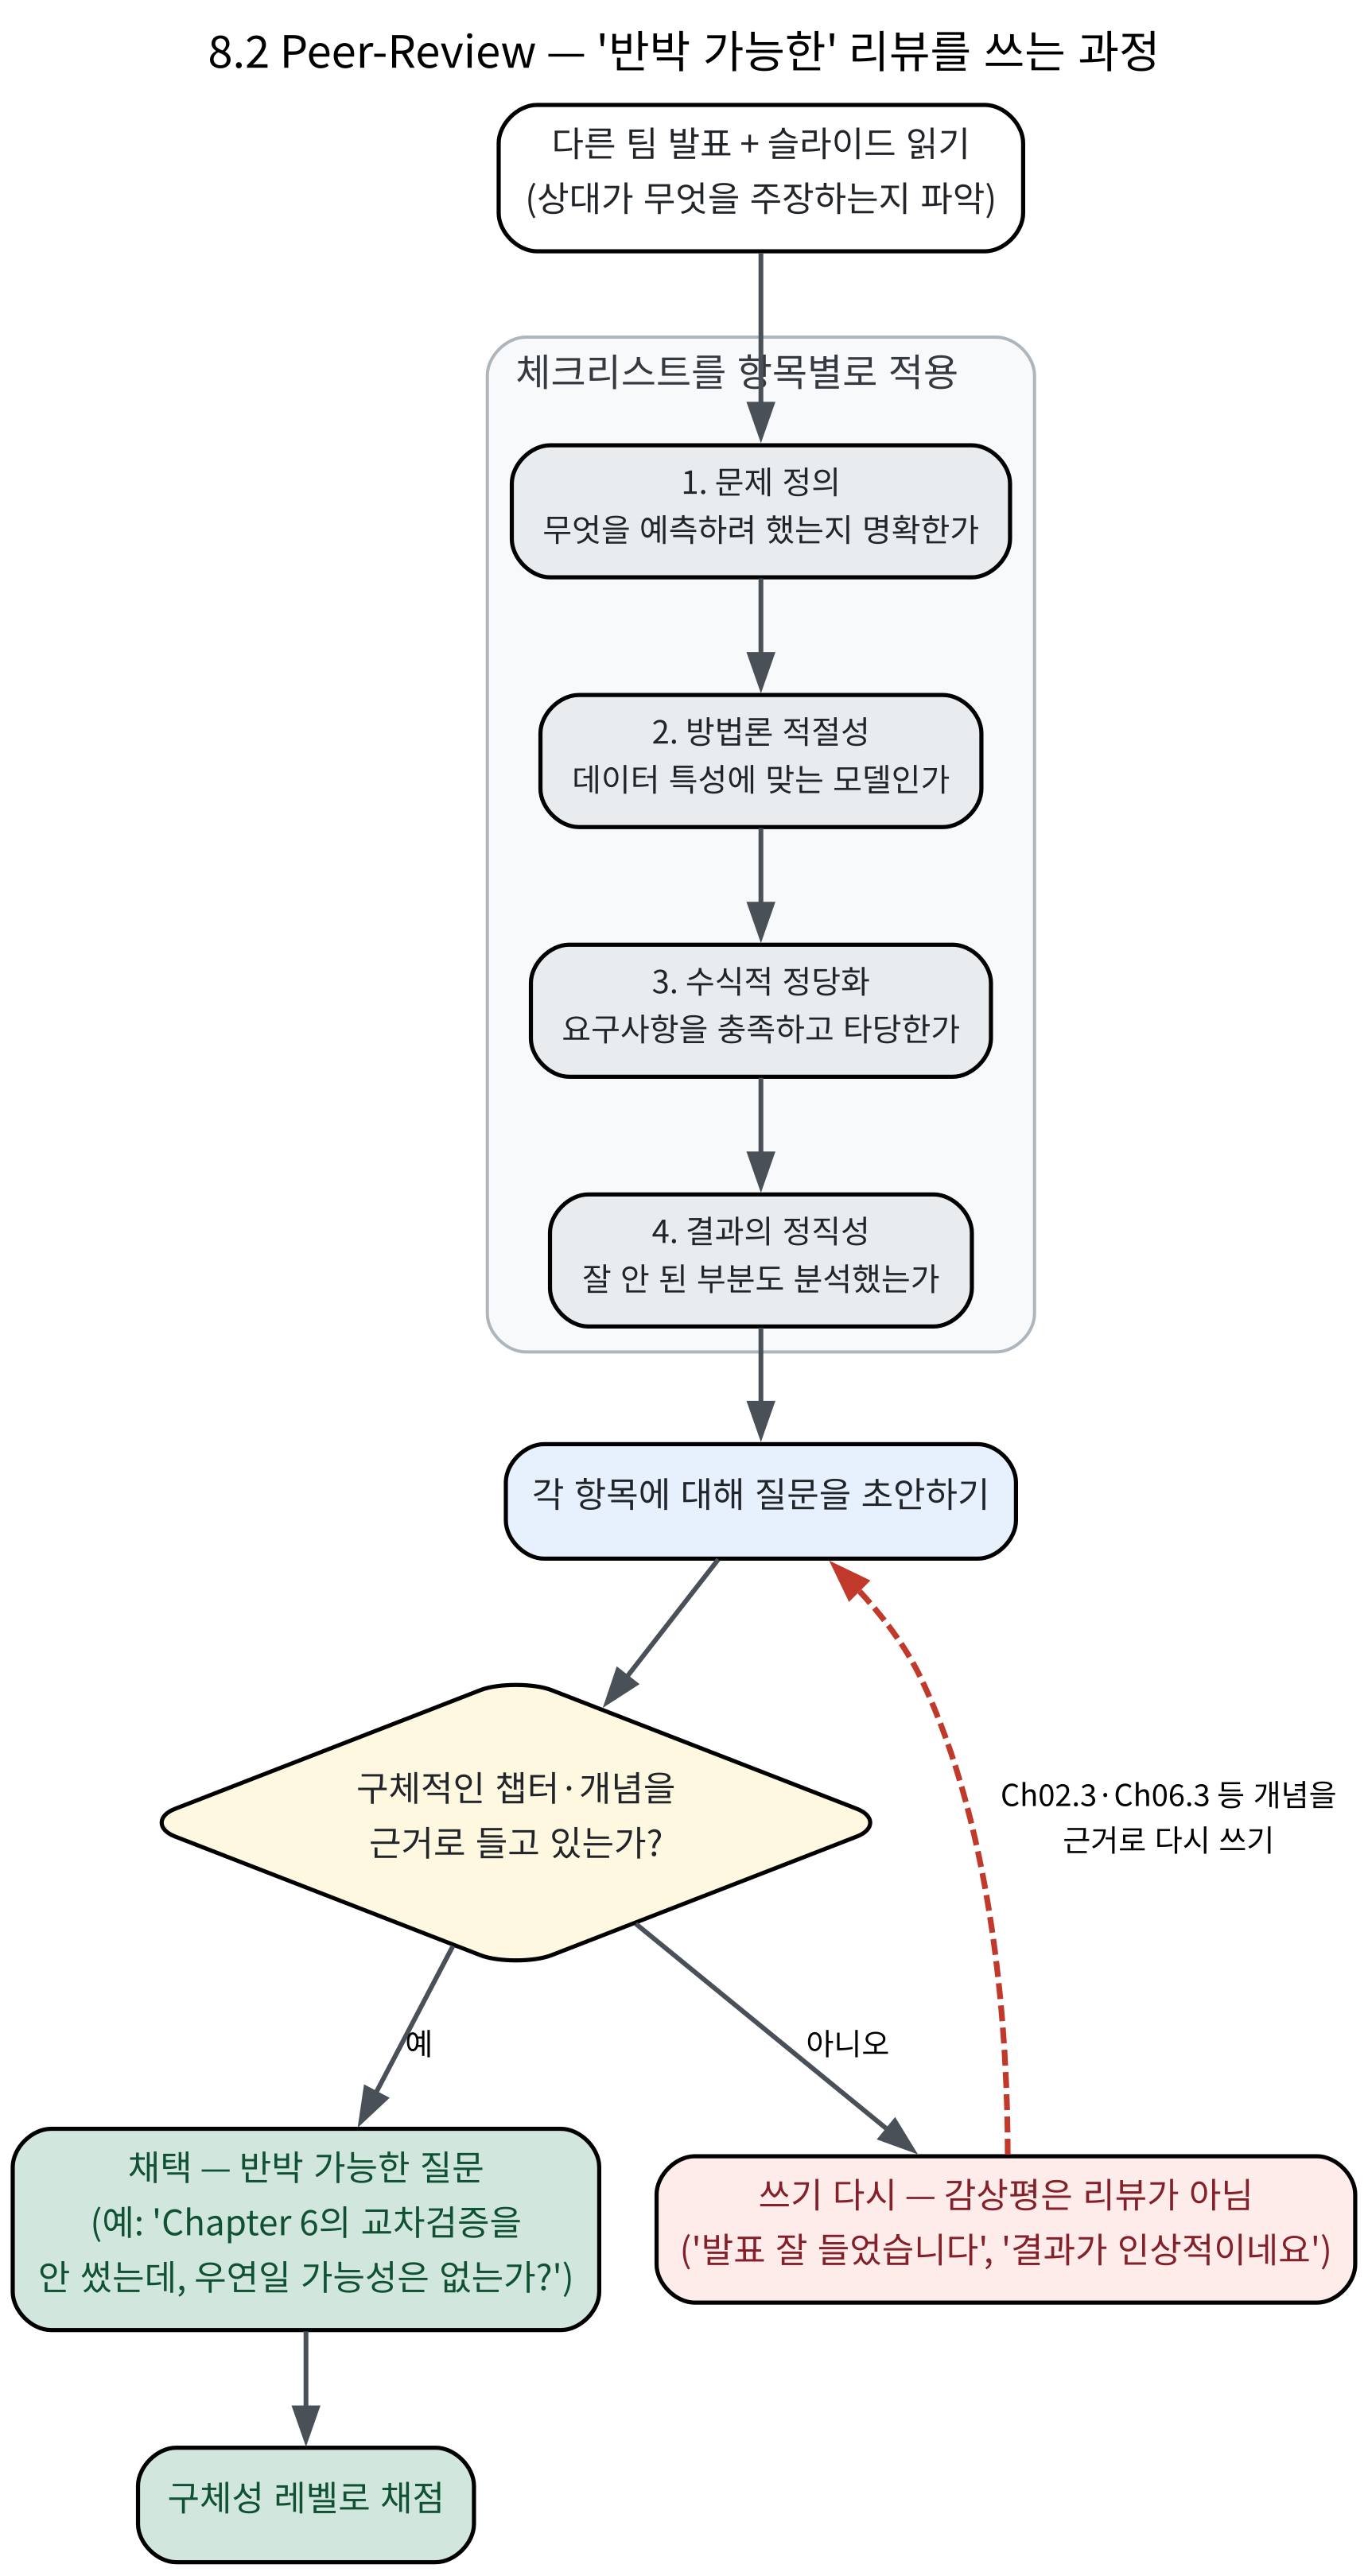
\includegraphics[width=\linewidth]{ch08_2_review_flow.png}
      {\footnotesize (1) 발표+슬라이드 읽고 주장 파악 $\to$ (2)
      체크리스트 4항목 적용 $\to$ (3) 각 항목에 질문 초안 $\to$
      (4) ``구체적 챕터·개념을 근거로 두는가?'' 예 $\to$
      반박 가능한 질문 채택(초록), 아니오 $\to$ 감상평(빨강)으로
      떨어지고 개념을 근거로 (3)으로 회귀.}
    \end{column}
    \begin{column}{0.40\textwidth}
      \kb{형식으로 고정한 흐름}
      \begin{enumerate}
        \item 발표 듣고
        \item 체크리스트 4항목 적용
        \item 각 항목에 \textbf{구체적 관찰} 기록
        \item 그것이 \textbf{이 학기 개념(장·절)}에 뿌리
          박은 질문인지 검사
        \item 아니면 다시 쓰기
      \end{enumerate}
    \end{column}
  \end{columns}
\end{frame}

\begin{frame}[fragile]{리뷰 템플릿 --- 빈칸이 채워지지 않으면 3점 미만}
\begin{lstlisting}
팀 이름: ________   리뷰어: ________
1. 문제 정의 -- 무엇을 예측/분류하려 했는지 한 문장. 명확했는가?
2. 방법론 적절성 -- 데이터의 어떤 특성(불균형, 차원, 결측치)에
   어떤 모델이 맞았는가? 그 선택에 동의하는가, 근거와 함께.
3. 수식적 정당화 -- "최소 1개"(8.1)를 채웠는가? 어떤 장의 개념을
   썼고, 그 설명이 *실제로* 타당한가?
4. 결과의 정직성 -- 잘 안 된 부분과 그 원인을 분석했는가?
5. 반박 가능한 질문 (필수, 1개 이상)
   근거 개념: Ch__ 절__ (개념: ______)
   질문: ________ (답이 나쁘면 결과가 흔들려야 한다)
\end{lstlisting}
  \vskip0.2em
  {\footnotesize 5번의 빈칸이 채워지지 않으면 리뷰는 1$\sim$2점에
  머문다 --- ``개념''과 ``질문'' 두 칸이 모두 비어 있어야
  \textbf{반박 불가능한} 리뷰다. 템플릿 채우기가 곧 ``구체적인가?''
  라는 채점 기준의 자기 점검.}
\end{frame}

\begin{frame}{자주 하는 실수: 리뷰가 감상평에 머무는 것}
  \begin{itemize}
    \item ``발표 잘 들었습니다'', ``결과가 인상적이네요'' ---
      체크리스트를 \textbf{형식적으로 채웠을 뿐}, 발표팀에게
      실제로 도움이 되는 정보를 전혀 주지 않는다.
    \item \textbf{구체적인 챕터·개념을 근거로 든 질문}만이
      ``반박 가능''하다 --- 발표팀이 답하려면 실제로 자신의
      결과를 다시 들여다봐야 하기 때문.
  \end{itemize}
  \vskip0.6em
  \begin{block}{채점의 축}
    peer-review 점수가 체크리스트를 ``채웠는가''가 아니라
    \textbf{``그 안의 질문이 얼마나 구체적인가''}로 매겨지는
    이유가 여기에 있다.
  \end{block}
\end{frame}

\begin{frame}{확인 문제 (1)}
  \begin{itemize}
    \item \textbf{1.} ``5\%만 양성인 데이터에 신경망을 써서 정확도
      95\%를 냈다''는 발표. 가장 약한 부분은? Ch.\,2.3 개념으로
      반박 가능한 질문 하나를 쓰시오.
      \vskip0.3em
      {\footnotesize \textbf{답}: 정확도의 함정(Ch02.3) ---
      \textbf{모두 음성}으로만 찍어도 95\%. 질문: ``Precision과
      Recall(또는 PR-AUC)이 각각 얼마인가요? 무조건 음성 모델과
      같은 수인데, 실제로 양성을 얼마나 더 잡는지 보여주세요.''}
    \item \textbf{2.} ``\textbf{테스트셋}으로 여러 $\lambda$ 중
      가장 좋은 것을 골랐다''고 인정한 팀. Ch.\,6.3의 어떤
      원칙이 깨졌고, 왜 그 숫자가 낙관적인가?
      \vskip0.3em
      {\footnotesize \textbf{답}: ``test를 하이퍼파라미터 선택에
      쓰지 말고 딱 한 번만'' 원칙 위반. 후보 중 \textbf{가장 잘
      나온 것}을 고르면 잡음의 max를 고르는 것 --- 후보가 많을수록
      낙관적으로 읽힘(선택 편향). 올바르게: val로 $\lambda$
      선택 후 test \textbf{한 번}.}
  \end{itemize}
\end{frame}

\begin{frame}{확인 문제 (2)}
  \begin{itemize}
    \item \textbf{3.} ``왜 반박 가능한(falsifiable) 질문이 좋은
      리뷰의 기준인가?'' 한 단락으로.
      \vskip0.3em
      {\footnotesize \textbf{답}: Popper의 반증주의처럼, 과학적
      주장은 ``틀렸음을 보이는 관측이 상상이 가능한가''로
      판별된다. 좋은 리뷰 질문도 발표팀이 \textbf{제대로 답하지
      못하면 결과가 무너지는} 질문이어야 한다. 감상평은 답이
      아무리 나빠도 결과를 흔들지 못함. peer-review는 Amgen처럼
      ``내 결과도 남이 재현·반박할 수 있는가''를 \textbf{미리
      방어}하는 과학적 행위.}
    \item \textbf{4.} ``모델 선정이 적절해 보이지 않습니다''는
      3단 채점 중 어디인가? 3점으로 \textbf{어떻게} 바꿀 수
      있는가?
      \vskip0.3em
      {\footnotesize \textbf{답}: 근거(개념, 데이터 특성)가 없으므로
      \textbf{2점}. 3점이려면 \textbf{관찰+개념+왜}를 채운다:
      ``99:1 불균형에서 정확도로 비교했는데(관찰), Ch02.3 함정으로
      '둘 다 항상 다수 클래스' 모델일 수 있어(개념)
      Precision·Recall 또는 PR-AUC로 다시 비교해야 합니다(왜).''}
  \end{itemize}
\end{frame}

\begin{frame}{확인 문제 (3) --- 어떤 숫자를 신뢰하는가}
  \begin{itemize}
    \item \textbf{5.} 95\% 불균형 데이터에서 ``test 정확도
      93\%''를 헤드라인으로, 그 뒤에 ``PR-AUC 0.55''도 함께
      보고한 팀. ``모델이 쓸모있는가''를 판단할 때 \textbf{어떤}
      숫자를 신뢰해야 하는가?
      \vskip0.3em
      {\footnotesize \textbf{답}: \textbf{PR-AUC 0.55} 쪽. 95\%
      불균형에서는 정확도 93\%가 \textbf{무조건 다수 클래스}
      모델(95\%)보다도 \textbf{낮다} --- 정확도는 이 모델이
      ``무조건 다수''보다 못하다는 뜻일 뿐, 유용성의 \textbf{크기}를
      말해주지 않는다. PR-AUC 0.55는 베이스레이트(0.05)보다
      훨씬 높아 ``우연보다 더 잘 잡고 있다''는 신호.
      \textbf{유용성}을 논할 때는 PR-AUC/재현율 기준.}
  \end{itemize}
  \vskip0.6em
  \begin{block}{판정 기준}
    정확도는 \textbf{순위를 정하는 데는}, PR-AUC/재현율은
    \textbf{유용성을 논하는 데는} 사용할 수 있다 ---
    두 숫자를 \textbf{둘 다} 보고, 불균형이 심할수록 후자에
    무게를 둔다.
  \end{block}
\end{frame}

\begin{frame}{자주 묻는 질문}
  \begin{itemize}
    \item \textbf{Q. 우리 팀 발표에 대한 리뷰가 너무 비판적이면?}
      비판적인 리뷰일수록 체크리스트의 목적에 가깝다 ---
      발표팀이 못 보고 지나친 문제를 찾아주는 것이지 인신공격
      이 아니다. 다만 리뷰어도 ``왜 그 지적이 타당한지''를
      \textbf{이 학기 개념으로 뒷받침}해야 한다.
    \item \textbf{Q. 시간이 부족하면 무엇을 우선?}
      \textbf{``방법론 적절성''}을 가장 먼저 --- 문제 정의가
      아무리 명확해도 데이터 특성에 안 맞는 모델(예: 불균형에
      정확도)을 골랐다면 뒤의 \textbf{결과 해석 전체}가
      흔들리기 때문.
    \item \textbf{Q. 발표팀이 ``좋은 지적입니다''만 하면?}
      그건 발표팀이 \textbf{아직 답하지 못했다는} 증거. 좋은
      리뷰는 ``좋은 지적''으로 넘길 수 \textbf{없는} 질문 ---
      답하려면 \textbf{새로운 계산·실험·그래프}를 꺼내야 하는
      질문. ``Precision·Recall을 보여주세요''는 그 자리에서
      혼동행렬을 다시 써야 답 $\to$ \textbf{반박 가능}.
      ``모델을 더 생각해보세요''는 어떤 답도 가능 $\to$ 반박
      불가능. ``좋은 지적''으로 끝나면 그 질문은 2점에 머문
      것 --- \textbf{구체적 산출물(어떤 그래프/계산)을 요구}하는
      쪽으로 재작성.
  \end{itemize}
\end{frame}

\section{8.3 중간고사 대비 총정리}

\begin{frame}{새 개념이 없다 --- ``재현 가능한가''를 점검한다}
  \begin{itemize}
    \item Block A(Ch.\,2--8)의 마지막 블록. 새 개념 \textbf{없음}
      --- 지금까지의 ``알고 있는 것''이 \textbf{시험장에서 빈
      종이에 스스로 재현}될 수 있는지 점검.
    \item ``수업에선 이해했다''와 ``시험장에서 유도할 수 있다''는
      서로 다른 역량 --- 손유도와 ``왜?'' 질문에서 후자가 직접
      점수로 연결.
  \end{itemize}
  \vskip0.5em
  \begin{block}{이 절의 구조}
    시험에서 가장 자주 나오는 질문 유형 \textbf{4개}를 뽑고,
    그중 \textbf{``손으로 써야 하는'' 3가지(유도 템플릿 ①②③)}를
    실제로 종이에 풀고, 나머지는 자가진단 플로우와 확인 문제
    9개로 채운다. 실습 노트북은 세 템플릿의 숫자를 코드로
    검증.
  \end{block}
\end{frame}

\begin{frame}{장별 핵심 질문 --- 자가진단 도구}
  \scriptsize
  \begin{tabular}{@{}cll@{}}
    \toprule
    장 & 핵심 질문 & 다시 봐야 할 개념 \\
    \midrule
    Ch02 & 같은 선형모델로 회귀와 분류를 어떻게 모두 푸는가
      & 경사하강법, 정규방정식, 교차 엔트로피 \\
    Ch03 & 생성적 접근과 판별적 접근의 차이는 무엇인가
      & 베이즈 정리, GDA/로지스틱회귀의 관계 \\
    Ch04 & ``가깝다''만으로 예측하는 것의 한계는 무엇인가
      & 편향-분산, 차원의 저주 \\
    Ch05 & 확률이 아니라 마진으로 경계를 정하면 무엇이
      달라지는가 & 서포트 벡터, 커널 트릭 \\
    Ch06 & 과적합을 손실함수로 어떻게 통제하는가
      & L1/L2 정규화, 교차검증 \\
    Ch07 & 트리를 어떻게 앙상블하고 예측을 어떻게 설명하는가
      & 정보이득, RF vs GBDT, SHAP \\
    \bottomrule
  \end{tabular}
  \vskip0.6em
  \begin{itemize}
    \item \textbf{목록으로 읽지 말고} ``핵심 질문''에 한 문장으로
      답할 수 있는가의 \textbf{자가진단 도구}로.
    \item 여섯 문항 전부 막힘없이 답하면 나머지는 빠르게 훑고,
      답이 끊기는 장은 ``다시 봐야 할 개념''으로 돌아가 확인
      문제 2$\sim$3개 --- 가장 효율적.
  \end{itemize}
\end{frame}

\begin{frame}{시험에서 반복되는 질문 유형 4가지}
  \small
  \begin{tabular}{@{}llp{6.4cm}@{}}
    \toprule
    유형 & 예 & 어디에서 준비하나 \\
    \midrule
    ① \kb{유도(빈칸 완성)} & ``경사하강 1스텝 빈칸 채우시오'',
      ``KKT에서 해를 구하시오'' & §유도 템플릿 ①② \\
    ② \kb{``X를 키우면?'' 정성 추론} & ``C를 크게 하면?'',
      ``$\lambda$를 0으로 하면?'', ``트리 깊이를 늘리면?''
      & §템플릿 ②③, §편향-분산 스펙트럼 \\
    ③ \kb{모델 비교(장 넘나들기)} & ``kNN과 SVM은 왜 둘 다
      스케일링이 필요한가?'', ``RF와 GBDT의 차이는?''
      & §확인 문제 1$\sim$6 \\
    ④ \kb{실전 코드·절차 판정} & ``이 파이프라인의 누수
      지점은?'', ``이 발표의 약점과 질문 하나'' & §누수 원칙,
      8.1·8.2절 \\
    \bottomrule
  \end{tabular}
  \vskip0.7em
  \begin{block}{시험 준비가 끝나는 구조}
    \kq{①②를 실제로 종이에 써보고, ③④는 기존 섹션(확인
    문제, ``자주 하는 실수'')을 훑으면 된다.}
  \end{block}
\end{frame}

\begin{frame}[allowframebreaks]{유도 템플릿 ①: 로지스틱회귀 경사하강 1스텝}
  \begin{block}{문제}
    1차원 입력, $n=3$ 샘플, $x=(1,2,3)$, $y=(0,1,1)$, 현재
    $w=0.1$, $b=0$, 학습률 $\eta=0.5$. 교차 엔트로피 손실
    \[ \ell = -\frac1n\sum_i \big[y_i\log\hat p_i + (1-y_i)\log(1-\hat p_i)\big]
       \qquad (\hat p_i=\sigma(wx_i+b)) \]
    에서 \textbf{경사하강 1스텝}을 손으로 수행하라. 4단계가
    \kb{예측 대입 $\to$ 손실 계산 $\to$ 경사 $\to$ 업데이트} ---
    손실이 무엇이든 이 순서만 지키면 같은 모양.
  \end{block}
  \vskip0.3em
  \textbf{1단계 — 예측 대입.} $z_i = wx_i+b = (0.1, 0.2, 0.3)$:
  \small
  \begin{center}
  \begin{tabular}{@{}lcccc@{}}
    \toprule
    샘플 & $x_i, y_i$ & $z_i$ & $\hat p_i=\sigma(z_i)$ & $\hat p_i - y_i$ \\
    \midrule
    1 & (1, 0) & 0.1 & 0.524979 & $+0.524979$ \\
    2 & (2, 1) & 0.2 & 0.549834 & $-0.450166$ \\
    3 & (3, 1) & 0.3 & 0.574443 & $-0.425557$ \\
    \bottomrule
  \end{tabular}
  \end{center}
  \textbf{2단계 — 손실 계산}(미분 전에 대수의 정확성 점검):
  \[ \ell = -\frac13\big[\log(0.475021)+\log(0.549834)+\log(0.574443)\big]
     = \frac{0.744436+0.597797+0.554336}{3} \approx 0.6322 \]
  \textbf{3단계 — 경사.} $\frac{\partial\ell}{\partial w}
  =\frac1n\sum_i(\hat p_i-y_i)x_i$ 에 대입:
  \[ \frac13\big[(+0.524979)(1)+(-0.450166)(2)+(-0.425557)(3)\big]
     = \frac{0.524979-0.900332-1.276671}{3} = -0.550675 \]
  $\frac{\partial\ell}{\partial b}=\frac13\sum_i(\hat p_i-y_i)
  =-0.116915$ 도 함께.
  \textbf{4단계 — 업데이트.}
  \[ w \leftarrow 0.1-0.5\times(-0.550675)=0.375338, \qquad
     b \leftarrow 0-0.5\times(-0.116915)=+0.058457 \]
\end{frame}

\begin{frame}{템플릿 ① ``왜?'': 부호 읽기와 $(\hat p-y)x$}
  \begin{itemize}
    \item \kb{부호 읽기}: 샘플 1은 실제 0인데 0.525로 예측 $\to$
      $(\hat p-y)>0$ --- 양수 기여가 $w$를 \textbf{작아지는} 쪽으로
      당김. 샘플 2·3은 실제 1인데 0.55·0.57 $\to$ 음수 기여로
      $w$를 \textbf{크는} 쪽으로 밀어올림.
    \item $x_i$가 곱하기 때문에 $x=3$인 샘플 3의 기여($-1.277$)는
      $x=1$인 샘플 1($+0.525$)의 \textbf{2.4배} ---
      ``크게 틀린'' 샘플이 아니라 \textbf{``큰 특징 값으로
      틀린'' 샘플이 더 강한 힘}. \textbf{이 부호·가중 해석 한
      줄}이 ``대입만 한 답''과 ``이해한 답''을 가른다.
    \item \kb{왜 $(\hat p-y)x$인가}(빈칸은 보통 여기): 연쇄법칙
      $\frac{\partial}{\partial w}[-\log\hat p]=-\frac1{\hat p}\cdot
      \frac{d\hat p}{dz}\cdot\frac{dz}{dw}$ 에
      $\frac{d\sigma}{dz}=\sigma(1-\sigma)$ 를 대입하면
      $\frac1{\hat p}\cdot\hat p(1-\hat p)=1-\hat p$ 로 시그모이드
      의 미분이 \textbf{정말 예쁜 형태}로 정리. ``시그모이드의
      미분이 \textbf{자신을 곱한 것}''이 이 깔끔함의 원인.
  \end{itemize}
  \vskip0.3em
  {\footnotesize 검증: $\ell(w)$를 $w$의 함수로 짜서 유한차분
  $\frac{\ell(w+\delta)-\ell(w-\delta)}{2\delta}$로 교차 검증하면
  $-0.550675$와 일치(실습 노트북 §1).}
\end{frame}

\begin{frame}[allowframebreaks]{유도 템플릿 ②: SVM KKT --- ``C가 실제로 바꾸는 것''}
  Ch.\,5.2 소프트 마진 SVM에서 ``C가 커지면 마진이 커진다''는
  \textbf{잘못된 직감}을 시험에서 확인하는 문제가 자주 나온다.
  \vskip0.4em
  \textbf{문제} --- 1차원 4개 점:
  \small
  \begin{tabular}{@{}clcl@{}}
    \toprule
    점 & $x$ & $y$ & 역할 \\
    \midrule
    A & $-1$ & $+1$ & \\
    B & $-1$ & $+1$ & A와 같은 위치(다중점) \\
    C & $+2$ & $-1$ & \\
    E & $-0.2$ & $-1$ & \textbf{이상치} --- $-1$인데 $+1$ 쪽에
      붙어 있음 \\
    \bottomrule
  \end{tabular}
  \vskip0.3em
  목적함수
  \[ \min_{w,b}\ \tfrac12 w^2 + C\sum_i \xi_i
     \qquad (\text{약분 } y_i(wx_i+b) \ge 1-\xi_i,\ \xi_i \ge 0) \]
  A·B가 같은 $(x,y)$이므로 대칭으로 $\alpha_A=\alpha_B\triangleq a$.
  \vskip0.4em
  \kb{KKT 세 조건} + 정합성:
  \begin{enumerate}
    \item \kb{$0 \le \alpha_i \le C$} --- $\alpha$는 ``점 $i$에게
      쓰인 위반 예산''. C가 전체 예산이면 $\alpha$는 각 점에
      배정된 몫.
    \item \kb{$\alpha_i \xi_i = 0$} --- 마진 위반($\xi_i>0$)을
      하는 점은 $\alpha$가 상한 C에 \textbf{꽉 차 있다}.
    \item \kb{$\alpha_i(y_if(x_i)-1+\xi_i)=0$}
      \begin{itemize}
        \item $\alpha_i=0$: 마진 바깥($y_if(x_i)\ge 1$), 해에
          영향 없음.
        \item $0<\alpha_i<C$: \textbf{마진 위에 정확히}
          ($y_if(x_i)=1$).
        \item $\alpha_i=C$: 마진 안 또는 오분류
          ($y_if(x_i)\le 1$).
      \end{itemize}
  \end{enumerate}
  \vskip0.3em
  \begin{block}{정합성 (stationarity)}
    \[ w = \sum_i \alpha_i y_i x_i, \qquad \sum_i \alpha_i y_i = 0 \]
    이 문제에선 클래스 2:2라 $\alpha_A+\alpha_B = \alpha_C+
    \alpha_E$. 이제 $C$를 0에서부터 올리며 각 구간의 해를 구한다.
    \kb{이 4구간 풀이(구간 경계 = ``어떤 $\alpha$가 상한/0에
    닿는가'')가 템플릿}.
  \end{block}
  \vskip0.3em
  \scriptsize
  \begin{tabular}{@{}cllll@{}}
    \toprule
    구간 & $C$ 범위 & $\alpha$ & $w, b$ & $\|w\|^2$, 마진
      $2/\|w\|$ \\
    \midrule
    I & $C \le \tfrac{10}{57}\approx0.175$
      & 전부 $=C$ & $(-3.8C,\ 1.9C)$ & $14.44\,C^2$; 마진
      $\tfrac{2}{3.8C}$ (52.6$\to$3.0) \\
    II & $\tfrac{10}{57}<C<\tfrac56$
      & $\alpha_E=C$, $a=\tfrac19+\tfrac{11}{30}C$,
        $\alpha_C=\tfrac29-\tfrac4{15}C$
      & \textbf{$(-\tfrac23,\ \tfrac13)$ 고정} &
      \textbf{4/9 고정}; 마진 \textbf{3.0 고정} \\
    III & $\tfrac56<C<\tfrac{25}{8}$
      & $\alpha_E=C$, $a=C/2$, $\alpha_C=0$ & $(-0.8C,\
        1-0.8C)$ & $0.64\,C^2$; 마진 $\tfrac{2.5}{C}$
      (3.0$\to$0.8) \\
    IV & $C \ge \tfrac{25}{8}=3.125$
      & $a=\tfrac{25}{16}$, $\alpha_E=\tfrac{25}{8}$,
        $\alpha_C=0$
      & \textbf{$(-\tfrac52,\ -\tfrac32)$ 고정} &
      \textbf{6.25 고정}; 마진 \textbf{0.8 고정} \\
    \bottomrule
  \end{tabular}
  \vskip0.4em
  {\footnotesize 구간 경계: I$\to$II는 A·B가 마진 위에 올 때까지
  $f(-1)=5.7C=1 \Rightarrow C=10/57$. II$\to$III은 $\alpha_C=0$이
  되는 $C=5/6$. III$\to$IV은 E가 마진 위에 오기까지
  $y_Ef(x_E)=0.64C-1=1 \Rightarrow C=25/8$. 참고: E는
  $C<25/16=1.5625$에서는 아직 \textbf{오분류} 상태.}
\end{frame}



\begin{frame}{4구간 읽는 법 (1): I·II --- 직감이 유일한 맞는 구간}
  \begin{itemize}
    \item \kb{구간 I} (C 작음): 예산이 작아 \textbf{모든 점}이
      상한 C에 꽉 참. 경계는 $x=0.5$에 고정($\pm1\cdot+2$ 군의
      중점)이고 C가 커지면 마진이 $C$에 비례해 \textbf{팽창}
      ($14.44C^2$) --- ``C를 올리면 마진이 커진다''는 직감이
      \textbf{유일하게} 맞는 구간.
    \item \kb{구간 II}: A·B가 마진 위에 닿자 ($C\approx0.175$)
      이상치 E의 위반($\xi_i>0$)이 $\alpha_i=C$로 최대 배정되고,
      경계는 $w=-\tfrac23,\ b=\tfrac13$ 으로 \textbf{정지}.
      마진 3.0은 +1 군($-1$)과 C($+2$) 사이의 최대 마진 ---
      \textbf{이상치를 무시하고 가능할 만큼} 큰 마진. 여기서 C를
      올려도 $\|w\|^2$는 4/9에서 \textbf{움직이지 않는다}.
  \end{itemize}
  \vskip0.4em
  \begin{block}{핵심}
    C가 바꾸는 것은 마진의 \textbf{크기}가 아니라
    \kq{``이상치 E의 위반을 얼마까지 사들이는가''}.
  \end{block}
\end{frame}

\begin{frame}{4구간 읽는 법 (2): III·IV + 실측}
  \begin{columns}[T]
    \begin{column}{0.50\textwidth}
      \begin{itemize}
        \item \kb{III}: E의 위반 비용이 커지자 ($C\ge5/6$)
          C($+2$)가 마진에서 빠짐($\alpha_C=0$), 경계가
          \textbf{왼쪽으로 미끄러지며} E를 감싸기 시작
          ($w=-0.8C$). 마진은 $\tfrac{2.5}{C}$로 \textbf{줄어든다}
          (C를 올리면 마진이 줄어드는 구간!). $C=25/16$에서
          E가 올바르게 분류.
        \item \kb{IV} ($C\ge3.125$): E도 마진 위에 닿으면 해는
          $w=-\tfrac52,\ b=-\tfrac32$ 로 \textbf{다시 정지} ---
          경계는 A($-1,+1$)과 \textbf{이상치 E}($-0.2,-1$)가
          정한다(중점 $-0.6$, 반갭 $0.4$, 마진 $0.8$).
      \end{itemize}
    \end{column}
    \begin{column}{0.48\textwidth}
      \centering
      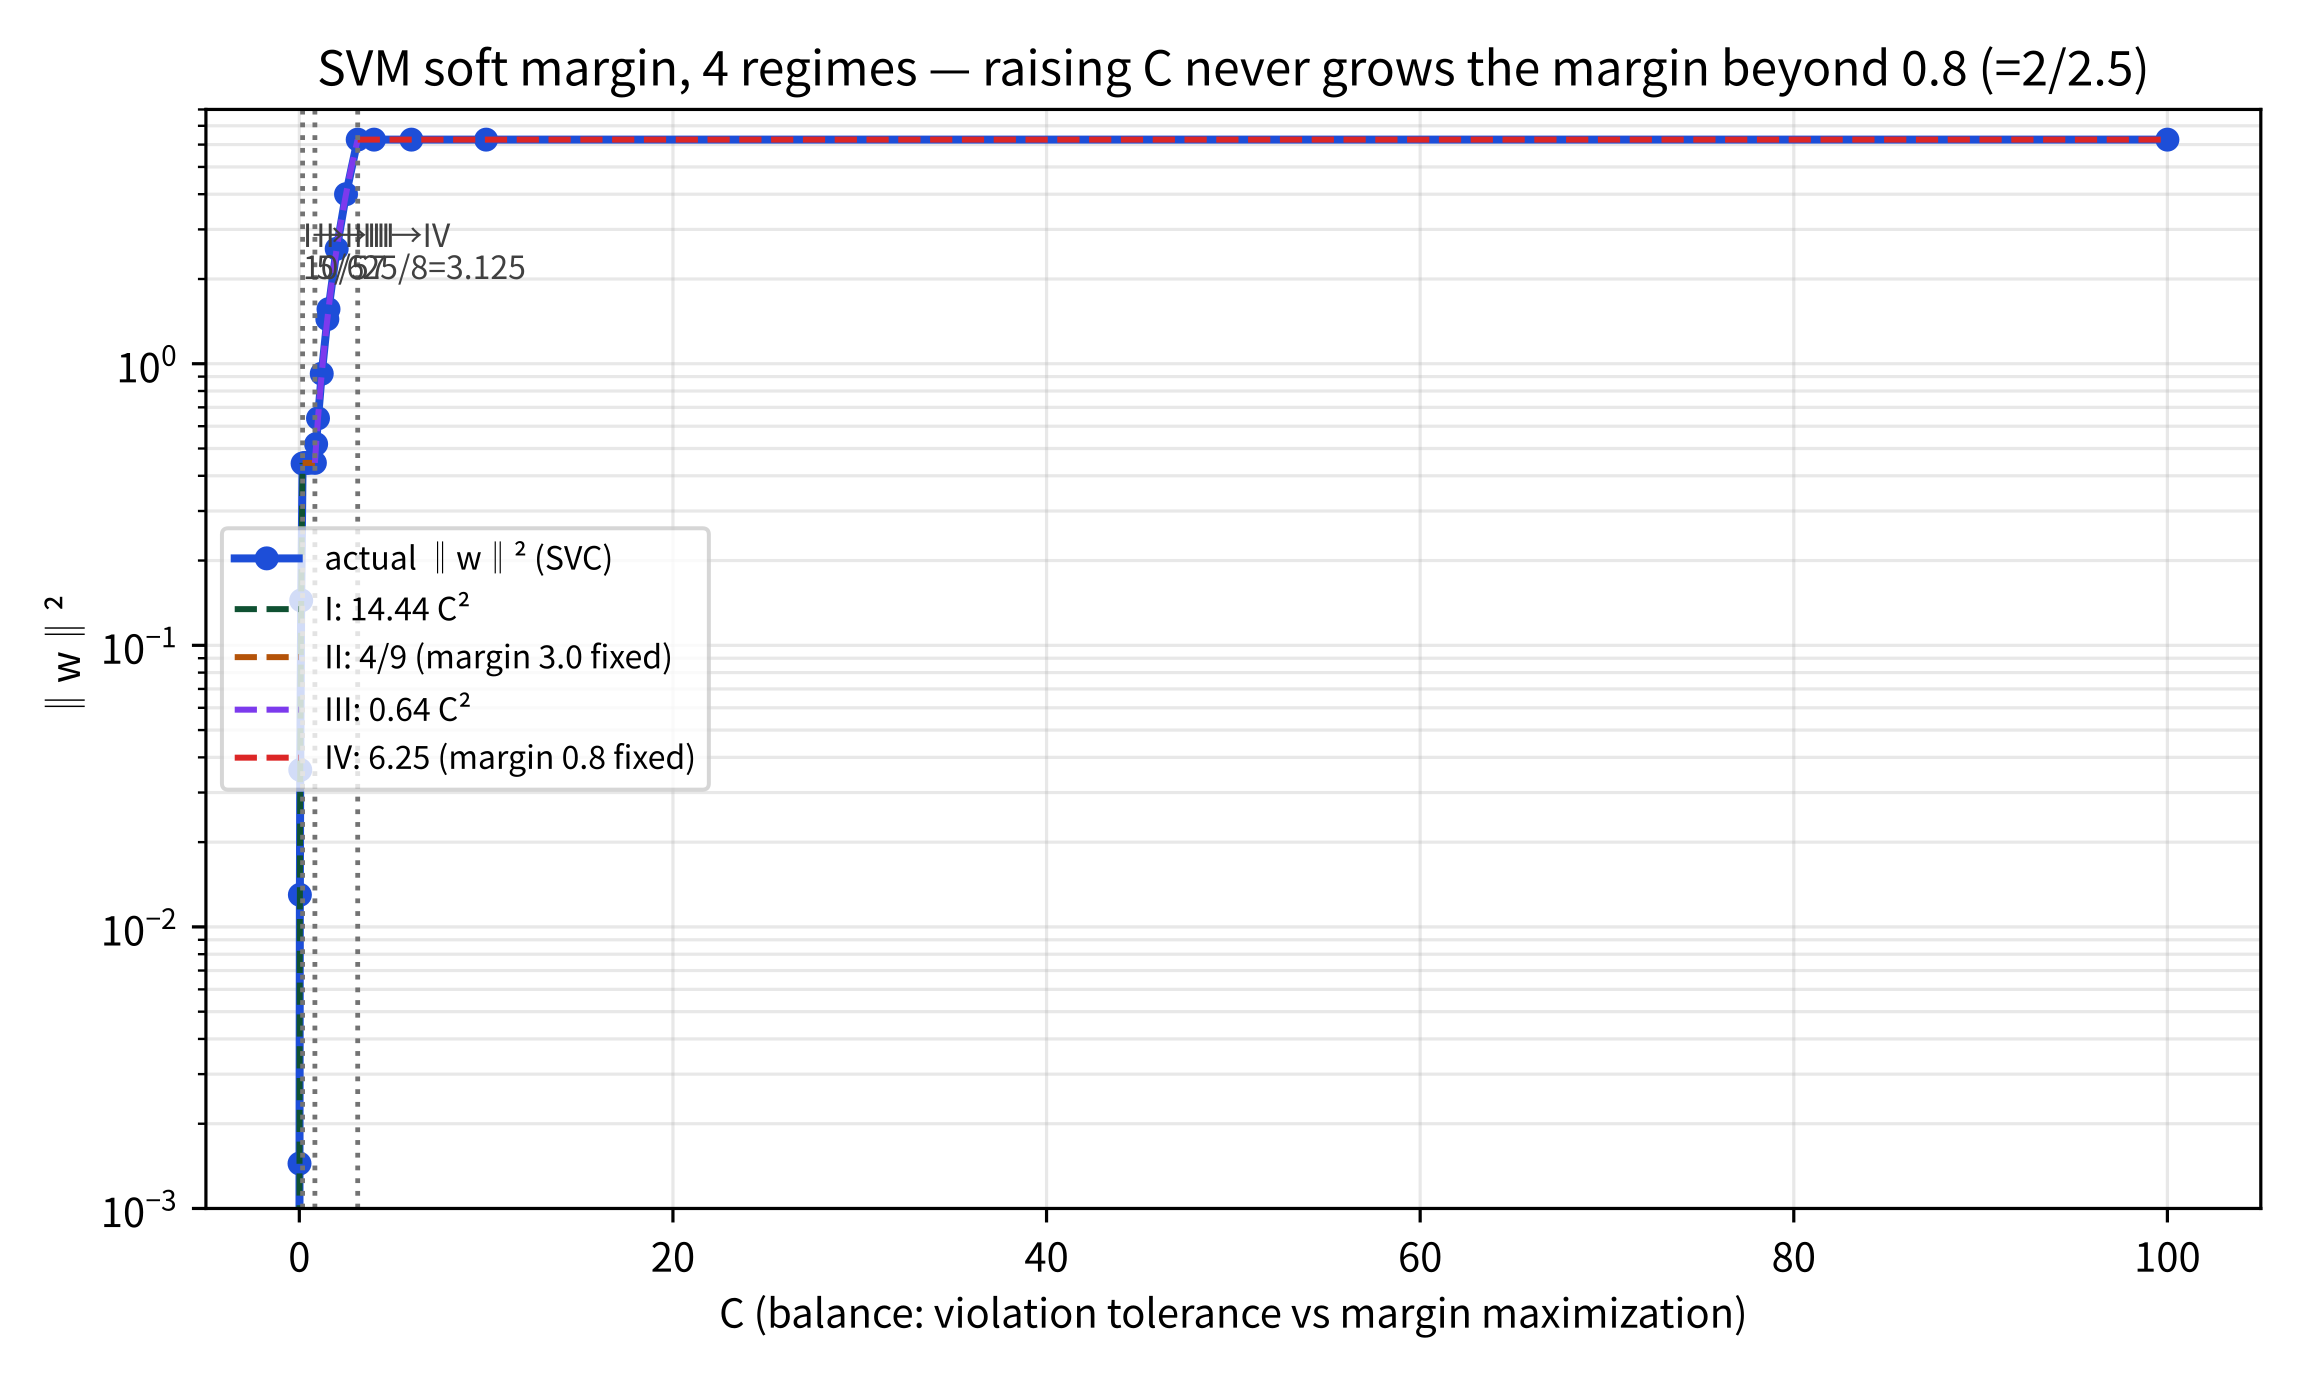
\includegraphics[width=0.96\linewidth]{ch08_3_svm_C_effect.png}
      {\footnotesize $C$를 0.0001$\sim$100으로 올리며 실제
      $\|w\|^2$(파랑)을 그린 것. 실선이 \textbf{두 번 꺾여 수평}
      (I: $14.44C^2$ $\to$ II: 4/9 $\to$ III: $0.64C^2$ $\to$
      IV: 6.25). 세 수직 점선($10/57,\ 5/6,\ 25/8$)이 구간
      경계. $C$를 아무리 올려도 $\|w\|^2$는 6.25를 넘지 않음.}
    \end{column}
  \end{columns}
  \vskip0.3em
  \kq{C를 100으로 올려도 $\|w\|^2=6.25$, 마진 0.8, 경계
  $x=-0.6$은 변하지 않는다.}
\end{frame}

\begin{frame}{템플릿 ②의 답안 뼈대}
  \begin{itemize}
    \item 시험에서 \textbf{``C를 크게 하면 무엇이 변하고 무엇이
      변하지 않는가''} --- 정답의 뼈대는 4구간표의 \textbf{구간
      IV}: \kq{``$C \ge C^*$ 이후 해는 $C$에 무관하다''}.
    \item 달성 가능한 마진의 범위는 \textbf{지오메트리가} 정한다
      --- 이상치를 무시하면 최대 3.0($-1$과 $+2$ 사이), 이상치를
      마진 안에 넣으려면 0.8($-1$과 $-0.2$ 사이)까지만 가능.
      C는 그 \textbf{두 극단 사이의 트레이드오프}를 선택할
      뿐, ``무한히 큰 마진''이라는 선택지는 존재하지 않는다.
    \item 실습 노트북 §2가 4구간표를 실제 $C$ 스위프로 검증
      ($\|w\|^2$가 $14.44C^2$로 오르면 4/9로 수평, $0.64C^2$
      로 다시 오르면 6.25로 수평), $\alpha_i$를
      \texttt{dual\_coef\_}로 읽어 손계산과 대조.
  \end{itemize}
\end{frame}

\begin{frame}{유도 템플릿 ③: ``두 항의 구조'' (적합도 + 단순성)}
  \scriptsize
  \begin{tabular}{@{}llll@{}}
    \toprule
    모델 & 목적함수 & 적합도 / 단순성 항 & 노브(트레이드오프) \\
    \midrule
    Ridge (Ch06) & $\ell_{\text{MSE}}+\frac{\lambda}{2}\|w\|^2$
      & $\ell_{\text{MSE}}$: 데이터에 맞추기 \; / \;
        $\|w\|^2$: 가중치 축소(분산$\downarrow$)
      & $\lambda$ (0$\to$무정규화, $\infty\to w=0$) \\
    Lasso (Ch06) & $\ell_{\text{MSE}}+\lambda\|w\|_1$
      & 위와 같음 \; / \; $\|w\|_1$: \textbf{정확히 0} 만드는
        켄(kink) & $\lambda$ \\
    소프트 마진 SVM (Ch05.2) & $\tfrac12\|w\|^2+C\sum_i\xi_i$
      & $C\sum\xi_i$: 위반 사들이기 \; / \;
        $\tfrac12\|w\|^2$: 마진 최대화
      & $C$ (0$\to w=0$, $\infty\to$하드마진) \\
    GBDT (Ch07.3) & (반복) 잔차에 트리 적합 + $\eta$로 축소
      & 트리: 잔차 설명 \; / \; $\eta$(학습률), $n$(트리 수)
      & $\eta$, $n$ \\
    kNN (Ch04) & \textit{(파라미터 없음 --- 전량 memorize)}
      & ``적합'' = 전량 암기 \; / \; $k$: 이웃 평균으로
        매끄럽게 & $k$ (1$\to$암기, $\infty\to$다수 클래스) \\
    \bottomrule
  \end{tabular}
  \vskip0.6em
  \begin{block}{패턴 한 줄}
    \kq{적합도 항은 ``데이터에 잘 맞추는 것'', 단순성 항은
    ``모델을 단순하게 유지하는 것''을 재고, 노브 하나가 둘의
    비중을 조절한다.}
  \end{block}
\end{frame}

\begin{frame}{템플릿 ③ 주의: 노브의 방향은 모델마다 반대}
  \begin{itemize}
    \item 노브를 0으로 가면 \textbf{적합만} 남고(과적합 위험,
      Ch.\,4.1), $\infty$로 가면 \textbf{단순성만} 남는다.
    \item 두 모델의 노브가 \textbf{역방향}인 점에 주의:
      Ridge의 $\lambda$는 ``크면 단순''인데, SVM의 $C$는
      \textbf{``크면 적합(위반을 덜 허용)''} ---
      ``$\lambda$를 크게 하면?''과 ``C를 크게 하면?'' 문항은
      \textbf{정반대 방향}으로 답해야 한다.
    \item kNN은 목적함수가 아예 \textbf{없으므로} 이 틀에 끼지
      않는다 --- ``kNN의 정규화 항은?''이라는 \textbf{함정 문항}
      의 정답: ``없다. $k$ 자체가 매끄러미(간접적 단순성)를
      조절할 뿐''.
  \end{itemize}
\end{frame}

\begin{frame}{편향-분산 스펙트럼: 같은 데이터, 네 모델}
  ``유연한 모델 vs 단순한 모델''을 \textbf{같은 데이터}에서
  놓고 train/val을 동시에 보는 문제는 Ch.\,4.1·6.2·7.3을
  한 문항에 끼워 넣는 전형. diabetes(442$\times$10)로
  train 265 / val 88 / test 89(스케일러 fit은 train으로만)를
  나눠 4개 모델 \textbf{실측}:
  \vskip0.4em
  \small
  \begin{center}
  \begin{tabular}{@{}lccc@{}}
    \toprule
    모델 & train R$^2$ & val R$^2$ & 격차 (train $-$ val) \\
    \midrule
    Ridge($\lambda{=}10^{-4}$) [Ch02,06] & 0.579 & 0.443 & 0.137 \\
    Ridge($\lambda{=}1$) [Ch06] & 0.579 & 0.442 & 0.137 \\
    kNN(k=5) [Ch04] & 0.618 & 0.329 & 0.290 \\
    Tree(무제한 깊이) [Ch07.1] & 1.000 & \textbf{$-0.014$}
      & \textbf{1.014} \\
    \bottomrule
  \end{tabular}
  \end{center}
  \vskip0.4em
  \begin{center}
  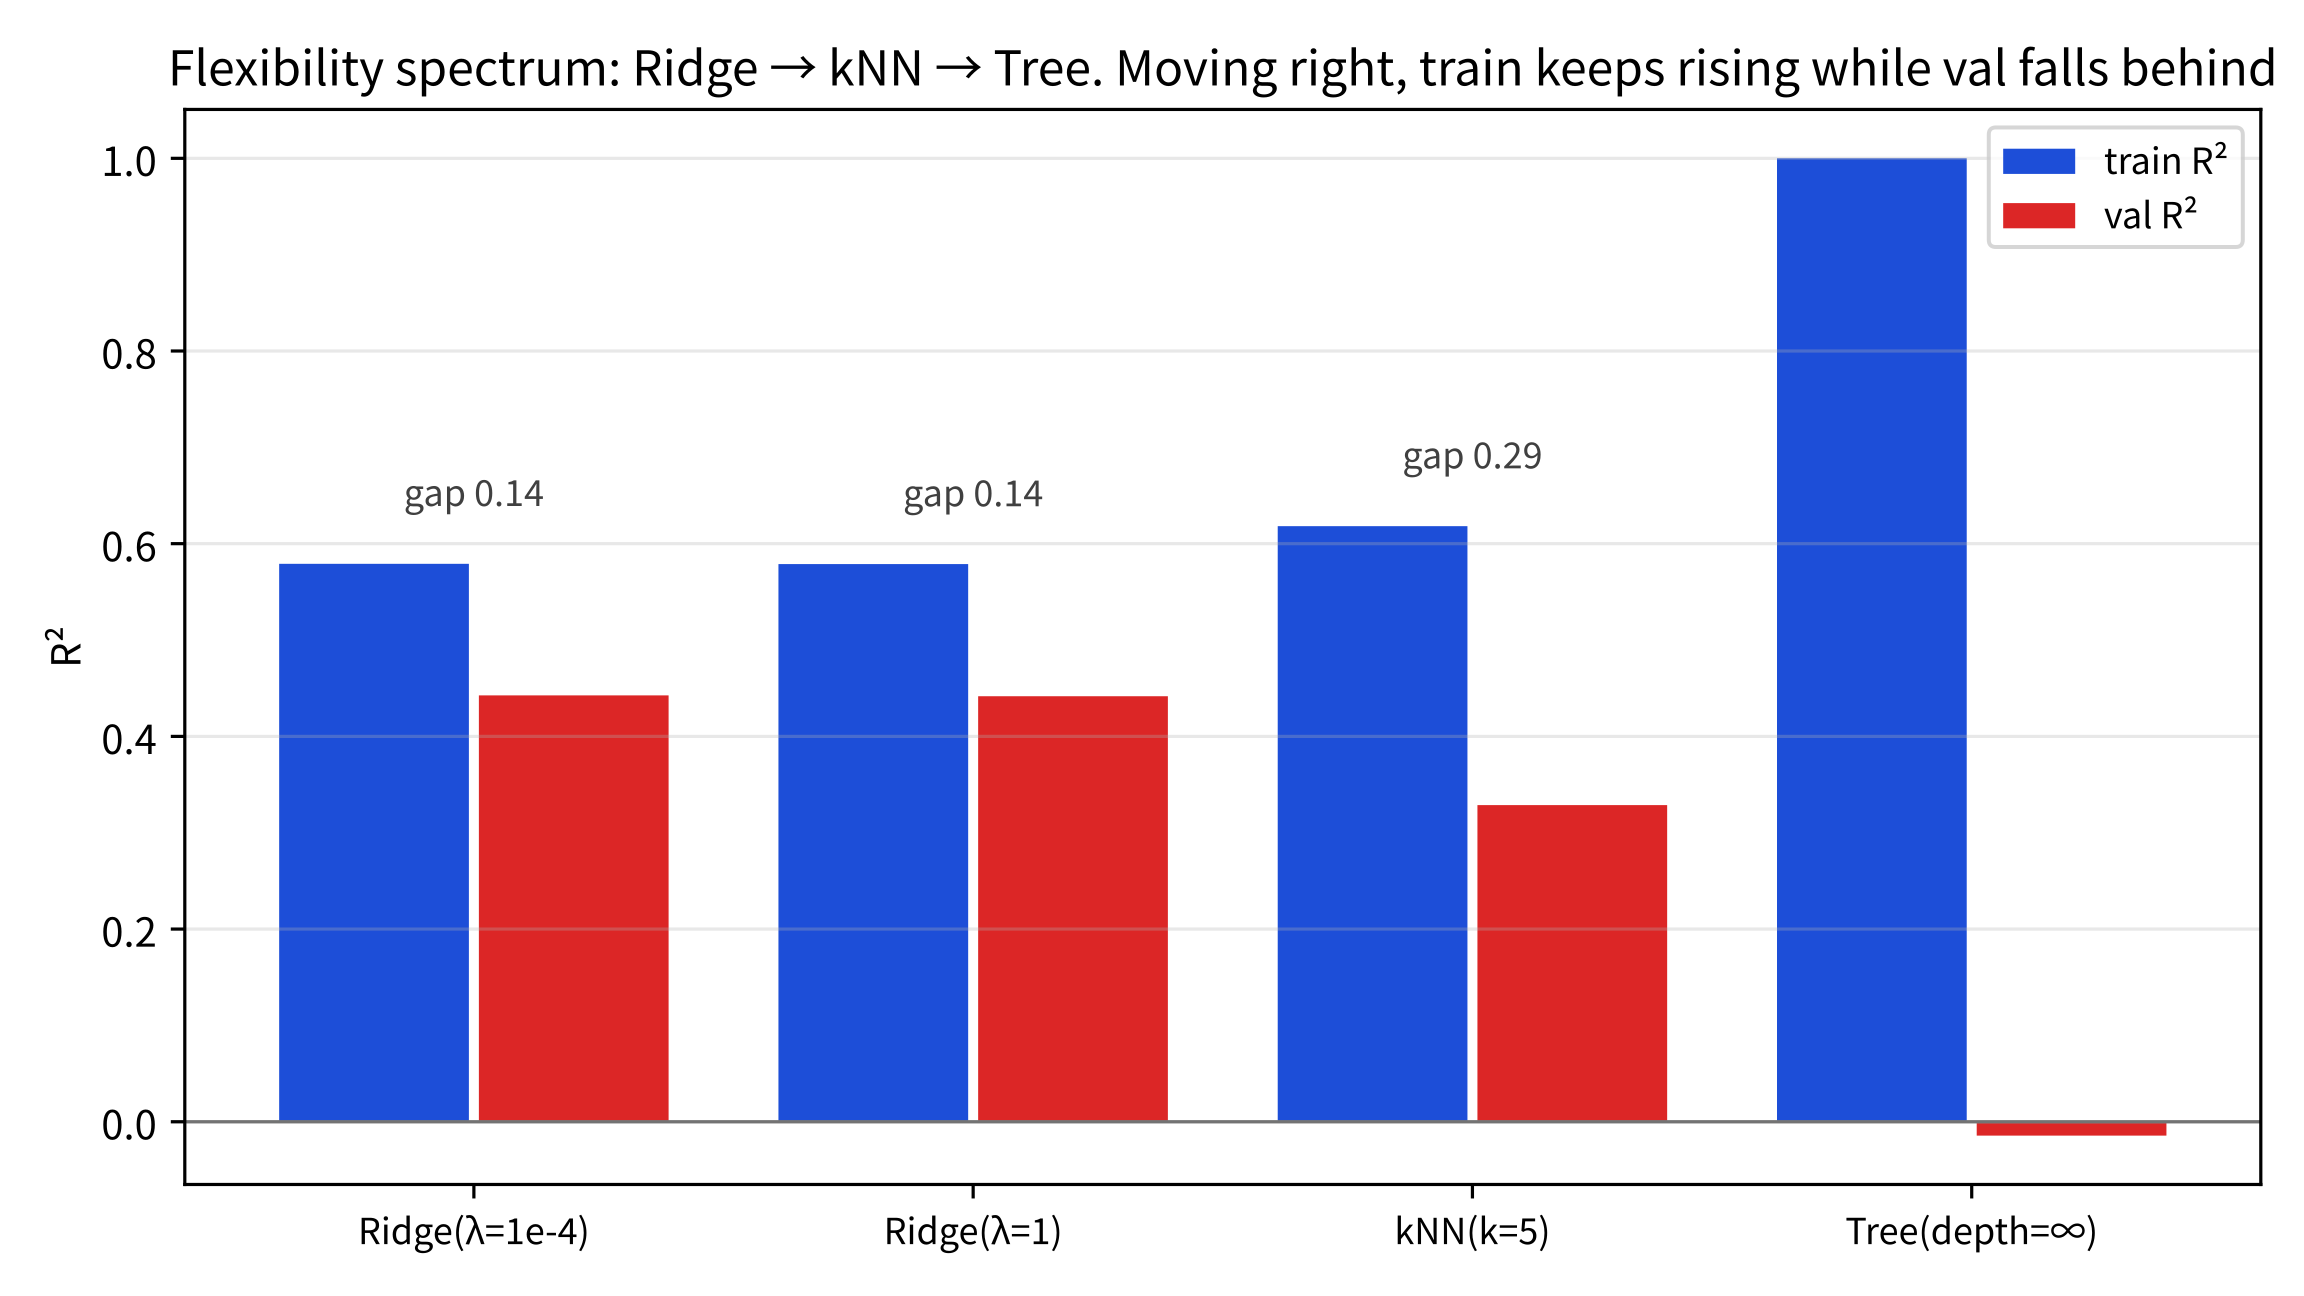
\includegraphics[width=0.90\linewidth]{ch08_3_model_spectrum.png}
  {\footnotesize 같은 diabetes 데이터에 네 모델의 train R$^2$
  (파랑)·val R$^2$(빨강) --- 왼쪽$\to$오른쪽으로 갈수록 train은
  올라가고 val은 벌어지며, 트리는 train 1.000인데 val이 0 아래
  ($-0.014$)로 처진다.}
  \end{center}
\end{frame}

\begin{frame}{스펙트럼 읽는 법 --- 시험 답안 구조}
  \begin{itemize}
    \item \kb{왼쪽 $\to$ 오른쪽으로 갈수록 모델의 유연성(가용
      자유도)이 커진다} --- Ridge는 10개 가중치에 $\lambda$로
      매달아 자유도를 조절하는 ``연속 스펙트럼''의 한 점,
      무제한 트리는 265건을 전부 외우는 ``스펙트럼의 끝''.
    \item 격차가 큰 모델(오른쪽)은 \textbf{분산}이 크다
      (Ch.\,4.1: ``모델 추정량이 train 데이터의 선택에 따라
      크게 흔들린다''). 격차가 작은 모델(왼쪽)은 \textbf{편향}
      이 크다 (Ch.\,6: ``평균적으로 진실을 향한 systematic한
      오차'').
  \end{itemize}
  \vskip0.4em
  \begin{block}{트리의 val R$^2$가 \textbf{0 아래}(음수)}
    train에서 1.000을 찍고도 검증 데이터에서는 \textbf{평균만
    예측하는 모델보다 나쁘다}는 뜻 --- Ch.\,6.2 U자 곡선의
    ``$\lambda\to0$ 쪽 끝''이 실제로 이렇게 처져 있음을
    보여주는 숫자. \kq{``train R$^2$=1.000이니까 좋은 모델''
    이라는 답안은 이 한 줄로 반박된다.}
  \end{block}
  \vskip0.3em
  {\footnotesize Ridge($10^{-4}$)와 Ridge(1)가 거의 같은 이유:
  표준화한 265개 샘플에서 $\lambda=1$은 데이터 스케일 대비
  \textbf{아직 매우 작은 벌금} --- ``$\lambda$가 1로 작아
  보이지만 실제로도 작을 수 있다''는 감각(Ch.\,6.1 스케일
  의존성). 교훈은 8.1절 GBDT 학습 곡선과 동일: \textbf{train
  곡선은 ``배운 것을'', val 곡선만 ``재는 것을'' 한다.}
\end{frame}

\begin{frame}{장을 넘나드는 동치성: GDA vs 로지스틱회귀}
  확인 문제 1의 답은 ``둘 다 $P(y{=}1\mid x)=\sigma(w^\top x+b)$
  라는 같은 \textbf{형태}에 도달한다''는 것이었다. ``동치''는
  어디까지 진실인가? breast\_cancer(569$\times$30)로
  \textbf{실측}(train/test 70/30, stratify, 스케일러
  train으로만):
  \small
  \begin{center}
  \begin{tabular}{@{}lc@{}}
    \toprule
    측정 & 값 \\
    \midrule
    로지스틱회귀 test AUC (판별적, Ch02) & 0.9934 \\
    GDA/LDA test AUC (생성적, Ch03) & 0.9855 \\
    두 모델의 test 출력 확률 상관계수 & 0.900 \\
    경계 벡터 방향 유사도 $\cos(w_{\text{logit}}, w_{\text{GDA}})$
      & 0.203 \\
    test 클래스 라벨 일치율 & 93.6\% \\
    \bottomrule
  \end{tabular}
  \end{center}
  \vskip0.3em
  \kb{결정 경계(분류)는 거의 같고}(라벨 93.6\% 일치, AUC 0.99
  부근), \kb{출력 확률도 꽤 비슷}하지만(상관 0.900),
  \kb{경계 벡터 $w$의 방향은 사실 다르다}($\cos 0.203$).
  \vskip0.2em
  Ch.\,3.2의 동치성은 \textbf{$P(x\mid y)$가 정규분포라는
  전제 하에} 성립하는 등식 --- 이 데이터가 정규분포가 아니므로
  전제가 \textbf{약하게 깨지고}, ``같은 \textbf{형태}의 경계,
  \textbf{다른 계수}''가 나온다.
  \vskip0.2em
  {\footnotesize \kq{시험의 3점 답안: 정규분포 가정이 성립하면
  계수까지 같은 방향의 경계, 전제가 깨지면 경계의 \textbf{형태}
  (시그모이드-선형)만 같고 계수는 경로(생성적 vs 판별적)에 따라
  다르다 --- 전제·반례 한 쌍이 있는 답.} ``동치''를 ``계수도
  같다''로 지나치게 확장하지 않는 것이 정직한 답안.}
\end{frame}

\begin{frame}{누수 원칙, 숫자로: 스케일러 fit의 위치}
  확인 문제 6의 ``가장 흔히 깨지는 지점'' ---
  \texttt{StandardScaler}의 \texttt{fit}(평균·표준편차)을
  \textbf{전체} 데이터로 하는 것 --- 의 효과를 diabetes(위
  스펙트럼과 같은 분할)에서 \textbf{실측}:
  \vskip0.4em
  \small
  \begin{center}
  \begin{tabular}{@{}lc@{}}
    \toprule
    스케일러 fit 범위 & val R$^2$ \\
    \midrule
    전체(train+val+test) --- \textbf{원칙 위반} & 0.4417 \\
    train만 --- 원칙 준수 & 0.4417 \\
    \bottomrule
  \end{tabular}
  \end{center}
  \vskip0.3em
  \begin{block}{차이는 $3\times10^{-5}$ --- ``거의 없다''가 정답}
    diabetes는 ``행 하나 = 독립 관측''이어서 train의
    평균/표준편차와 전체의 것이 거의 같다. 누수가 \textbf{크게}
    벌어지는 것은 Ch.\,6.3의 환자 예처럼 \textbf{동일 실체
    (환자, 계좌, 사용자)가 train과 val/test에 동시에 들어와
    정보를 공유할 때}다 --- 그때는 \texttt{fit}의 위치가
    아니라 \textbf{분할 자체}가 문제를 만든다.
  \end{block}
  \vskip0.3em
  \kq{시험 판정 기준: ``누수가 커지는 조건(공유된 실체, 시간
  순서)을 설명할 수 있는가''.}
\end{frame}

\begin{frame}{자가진단 5문항 + 40분 모의 문제}
  시험 1주일 전, \textbf{종이에} 답할 수 있다면 핵심은 잡은 것:
  \begin{enumerate}
    \item 장별 핵심 질문 6문항 중 \textbf{한 문장도 멈추지 않고}
      답할 수 있는 것이 몇 개인가? (5개 이상이면 양호)
    \item 템플릿 ①의 4단계를 \textbf{빈칸 없이} 쓸 수 있는가?
      ($\hat p$ 대입 $\to$ $\ell$ 계산 $\to$ $\frac1n\sum
      (\hat p-y)x$ $\to$ $w-\eta\nabla$, 숫자 $-0.5507$까지)
    \item 템플릿 ②에서 ``$C\ge25/8$ 이후 왜 $\|w\|^2=6.25$로
      고정되는가''를 \textbf{KKT 세 조건}으로 쓸 수 있는가?
    \item ``train R$^2$ = 1.000''인 모델에 대해 \textbf{편향-분산
      언어로 2문장 진단}을 쓸 수 있는가?
    \item 8.2절 가상 발표(99.8:0.2, 99.7\% vs 99.8\%)에 대해,
      \textbf{장·절을 명시한} 반박 가능한 질문 하나를 쓸 수
      있는가?
  \end{enumerate}
  \vskip0.3em
  {\footnotesize \textbf{40분 모의}: ① 유도 1문항 12분(시계
  보며) $\to$ ② ``C/$\lambda$를 키우면'' 8분 $\to$ ③ 장
  넘나들기 8분 $\to$ ④ 코드 판정 6분 $\to$ ⑤ 남은 6분 ②의
  답을 \textbf{반대로}(C를 0으로 하면?) 다시 쓰기. ⑤를 할 수
  있으면 \textbf{``노브 트레이드오프'' 양방향 이해가 완성}.}
\end{frame}

\begin{frame}{자주 하는 실수 6가지}
  각각 ``왜''를 빠뜨린 실수다:
  \begin{enumerate}
    \item \kb{경사 부호/계수 혼동}(①): $w\leftarrow w-\eta\nabla$
      의 \textbf{마이너스}나 $1/n$을 빼먹어 숫자가 $n$배로
      틀림($-0.5507$이 아니라 $-1.652$ = $1/n$ 누락).
    \item \kb{``C를 키우면 마진이 무한히 커진다''}(②): 구간 IV
      --- $C\ge3.125$ 이후 $\|w\|^2$는 \textbf{6.25로 고정}.
      ``C가 바꾸는 것은 위반 허용(어떤 점이 SV인가)이지
      \textbf{마진의 상한은 아니다}.''
    \item \kb{``동치''를 ``계수가 같다''로 확장}(§동치성):
      정규분포 전제가 깨지면 경계의 \textbf{형태}만 같고 $w$
      방향은 다르다($\cos 0.203$). 답안에 ``전제'' 한 단어가
      없으면 2점.
    \item \kb{``train R$^2$ = 1.000이면 좋은 모델''}(§스펙트럼):
      무제한 트리는 train 1.000 / val $-0.014$ ---
      \textbf{val(또는 gap)로만 판단}.
    \item \kb{스케일러를 전체로 fit하면서 ``깨끗해서 차이가
      안 났을 뿐''이라고 넘어감}(§누수): 환자/계좌 단위
      데이터에서는 격차가 커진다 --- ``누수가 커지는
      \textbf{조건}''을 함께 써야 만점.
    \item \kb{Ridge $\lambda$와 SVM $C$를 같은 방향의 노브로
      생각}(③): $\lambda$는 ``크면 단순'', $C$는 ``크면 적합''
      --- \textbf{정반대}. ``노브를 크게 하면'' 문항에서
      \textbf{가장 흔한 0점}.
  \end{enumerate}
\end{frame}

\begin{frame}[allowframebreaks]{확인 문제 1$\sim$4: 장 넘나들기}
  \begin{itemize}
    \item \textbf{1.} 로지스틱회귀(Ch02)와 GDA(Ch03)는 둘 다
      \textbf{어떤 공통된 최종 형태}에 도달하는가?
      \vskip0.2em
      {\footnotesize \textbf{답}: 둘 다 $P(y{=}1|x)=\sigma(w^\top x+b)$
      라는 \textbf{같은 시그모이드-선형 형태}(Ch03.2). 다만
      로지스틱회귀는 \textbf{판별적으로} 직접 학습하고, GDA는
      정규분포를 가정한 \textbf{생성적 모델링}에서 베이즈
      정리로 유도해내는 \textbf{경로}가 다르다.}
    \item \textbf{2.} kNN(Ch04)에서 $k$를 1로 두는 것과 SVM(Ch05)
      에서 $C$를 매우 크게 두는 것은 편향-분산 관점에서 어떤
      \textbf{공통점}이 있는가?
      \vskip0.2em
      {\footnotesize \textbf{답}: 둘 다 모델을 데이터에 최대한
      정확히 맞추려는 \textbf{극단} --- \textbf{분산이 커지고}
      (과적합 위험) 편향은 작아지는 쪽. $k=1$은 노이즈 하나에도
      민감하고, $C$가 매우 크면 이상치 하나까지 완벽히 분류하려
      든다(Ch05.2).}
  \end{itemize}

  \begin{itemize}
    \item \textbf{3.} Ridge(Ch06)와 소프트 마진 SVM(Ch05.2)
      목적함수는 둘 다 ``두 항의 합''. 각각 어떤 두 항인가?
      \vskip0.2em
      {\footnotesize \textbf{답}: Ridge는 ``적합도(원래 손실) +
      $\lambda\times$가중치 크기'', SVM은
      ``$\frac12\|w\|^2$(마진 최대화) + $C\times$위반 정도(힌지
      손실)''. 둘 다 ``데이터에 잘 맞추기''와 ``단순하게
      유지하기'' 사이 트레이드오프를 \textbf{하나의
      하이퍼파라미터}($\lambda$ 또는 $C$)로 조절.}
    \item \textbf{4.} 나이브베이즈(Ch03.3)와 결정 트리(Ch07.1)는
      \textbf{왜 둘 다} 특징 스케일링이 필요 없는가?
      \vskip0.2em
      {\footnotesize \textbf{답}: 나이브베이즈는 각 특징의 확률
      $P(x_j|y)$를 \textbf{독립적으로} 추정할 뿐 값들 사이의
      \textbf{거리를 재지} 않는다. 결정 트리는 ``이 특징이
      threshold보다 큰가''라는 \textbf{순서 정보}만 쓴다(Ch07.1
      FAQ) --- 둘 다 kNN·SVM·k-means처럼 거리를
      직접 계산하지 않기 때문.}
  \end{itemize}
\end{frame}


\begin{frame}[allowframebreaks]{확인 문제 5$\sim$7: 장 넘나들기 + 템플릿 ②}
  \begin{itemize}
    \item \textbf{5.} RF(Ch07.2)와 GBDT(Ch07.3)의 트리 학습
      방식(\textbf{독립 병렬} vs \textbf{순차적 잔차 학습})
      차이가, \textbf{라벨링 오류에 대한 취약성}에 어떤
      영향을 주는가?
      \vskip0.2em
      {\footnotesize \textbf{답}: RF는 트리들이 서로 \textbf{독립}
      적이라 한 트리가 라벨 오류를 과하게 학습해도 \textbf{다수결}
      에서 다른 트리에 의해 희석. GBDT는 각 트리가 이전까지의
      \textbf{잔차를 좇으므로}, 라벨 오류가 만드는 이상한
      잔차를 후속 트리들이 계속 따라가며 \textbf{과적합할
      위험}이 더 크다(Ch07.3 FAQ).}
    \item \textbf{6.} Ch.\,6.3의 데이터 누수(leakage) 원칙이
      이번 프로젝트에서 \textbf{가장 흔히 깨지는 지점}은?
      \vskip0.2em
      {\footnotesize \textbf{답}: 정규화·표준화 통계량(평균,
      표준편차)이나 결측치 대체값을 train/val/test로 나누기
      \textbf{전에 전체 데이터로} 미리 계산하는 경우(Ch06.3)
      --- \texttt{fit}은 반드시 \textbf{train에만} 적용하고,
      val/test에는 \texttt{transform}만 적용.}
  \end{itemize}

  \begin{itemize}
    \item \textbf{7.} 템플릿 ②의 4점 문제에서, $C=3.125$와
      $C=100$의 해($w^\star, b^\star$, SV 집합)는 \textbf{같다}.
      KKT 조건으로 \textbf{왜} 같은지, 그리고 $C$를 더 키워도
      바뀌지 않는 마진의 \textbf{상한 값(0.8)}을 두 점의
      지오메트리에서 직접 구해보자.
      \vskip0.2em
      {\footnotesize \textbf{답}: $C\ge25/8$에서는 A·B($-1,+1$)
      과 이상치 E($-0.2,-1$)가 \textbf{모두 마진 위에} 있고
      ($0<\alpha_i<C$), C($+2$)는 \textbf{마진 바깥}
      ($\alpha_C=0$) --- 이 세 상태(마진 위/위/바깥)는 $C$의
      \textbf{크기에 의존하지 않으므로} KKT의 해도 $C$에 무관.
      마진의 상한은 \textbf{가장 가까운 다른 클래스 두 점}이
      정한다: A($-1,+1$)과 E($-0.2,-1$) 사이의 \textbf{거리
      0.8}이므로 경계는 중점 $-0.6$, 반갭 $0.4$, 마진
      $2/\|w\|=0.8 \Rightarrow \|w\|=2.5,\ \|w\|^2=6.25$.}
  \end{itemize}
\end{frame}


\begin{frame}[allowframebreaks]{확인 문제 8$\sim$9: 템플릿 ①③}
  \begin{itemize}
    \item \textbf{8.} 템플릿 ①에서 학습률을 $\eta=0.5$ 대신
      $\eta=2$로 쓰면 1스텝 후의 $w, b$는? ``학습률을 크게
      하면 항상 빨리 수렴한다''가 왜 \textbf{성급한 결론}인지,
      이 숫자만으로 말할 수 있는 한계는?
      \vskip0.2em
      {\footnotesize \textbf{답}: $w=0.1-2\times(-0.550675)
      =1.201350$, $b=0-2\times(-0.116915)=0.233830$ --- 스텝이
      \textbf{정확히 4배}. 한계: 손실면이 볼록(교차 엔트로피는
      볼록)이므로 이 방향의 큰 스텝은 손실을 \textbf{낮추기는}
      한다, 그러나 스텝이 경사 변화율에 비해 너무 크면 다음
      스텝에서 반대쪽으로 \textbf{오버슈팅}하며 손실이
      튀어오를 수 있다 --- 1스텝만으로는 ``수렴''이 아니라
      ``더 큰 스텝''만을 볼 수 있다. (Ch09 Block B에서 학습률
      스케줄링이 이 주제의 일반화.)}
  \end{itemize}

  \begin{itemize}
    \item \textbf{9.} Lasso(Ch06.1)의 목적함수 두 항을 쓰고,
      ``왜 L1은 가중치를 \textbf{정확히 0}으로 만들지만 L2는
      (유한한 $\lambda$에서는) 그렇지 않은가''를 한 문장으로
      답하자.
      \vskip0.2em
      {\footnotesize \textbf{답}:
      $\min_w \ell_{\text{MSE}}(w) + \lambda\|w\|_1$.
      $\|w\|_1$은 $w_j=0$에 \textbf{켄(kink)}을 만들어, 원래
      손실 기울기의 절댓값이 $\lambda$ 이하이면 정답이 그 켄
      에 딱 붙어 $w_j=0$이 된다(Ch06.1의 소스 스로싱
      $\mathcal{T}_\lambda$). 반면 $\|w\|^2$은 0에서 \textbf{기울기
      가 0인 매끄러운} 볼록함수라 $w_j$를 0으로 \textbf{가까이
      당기지만} 유한한 $\lambda$로는 정확히 0까지 데려가지
      못한다.}
  \end{itemize}
  \vskip0.5em
  \begin{block}{이번 프로젝트가 남기는 교훈}
    \kq{지금까지 배운 어떤 모델도 ``항상 최선''이지 않다 ---
    실전에서는 데이터의 특성을 보고 어떤 도구를 쓸지
    \textbf{스스로 판단}해야 한다.}
  \end{block}
\end{frame}


\begin{frame}{자주 묻는 질문 + 시험 전날 세 숫자}
  \begin{itemize}
    \item \textbf{Q. 코딩 문제도?} Ch.\,2, 6, 7에서 반복 연습한
      \textbf{``핵심 줄이 빈칸으로 남겨진 함수를 완성하라''}
      형식이 가장 가까운 연습.
    \item \textbf{Q. 여섯 장을 전부 같은 비중으로?} 아니다 ---
      ``핵심 질문''에 스스로 답할 수 있는지가 \textbf{가장 빠른
      자가 진단}. \textbf{손유도 문제}(정규방정식,
      GDA$\leftrightarrow$로지스틱회귀 동치성, 마진 공식)는
      그대로 다시 나올 가능성이 높아 우선순위 고.
    \item \textbf{Q. ``장 넘나들기'' 연습법?} 한 문항을
      \textbf{두 장의 언어로 각 한 문장씩} --- 예: 확인 문제 4는
      ``Ch03.3의 언어: $P(x_j\mid y)$를 독립 추정하므로 거리
      계산이 없다'' + ``Ch07.1의 언어: 순서($>$threshold)만
      쓰므로 스케일에 불변''.
  \end{itemize}
  \vskip0.4em
  \small
  \begin{center}
  \begin{tabular}{@{}ll@{}}
    \toprule
    시험 전날 \textbf{세 숫자} & 의미(장) \\
    \midrule
    $-0.5507$ & 템플릿 ①의 1스텝 경사 (Ch02) \\
    $C^*=3.125$ 이후 $\|w\|^2=6.25$ 고정 & 템플릿 ②의 마진
      상한 0.8 (Ch05) \\
    무제한 트리: train 1.000 / val $-0.014$, 격차
      $\approx1.0$ & §스펙트럼 (Ch04·06·07) \\
    \bottomrule
  \end{tabular}
  \end{center}
  {\footnotesize 세 숫자를 ``어떤 가정에서, 왜'' 나오는 수로
  설명할 수 있으면 유도 문제의 뼈대는 확보 --- 숫자 자체는
  실습 노트북에서 언제든 재현.}
\end{frame}

\begin{frame}{이번 주차 정리}
  \begin{enumerate}
    \item \kb{8.1 팀 프로젝트} --- 4주 파이프라인
      (문제 정의 $\to$ 3분할·train-fit·모델 비교 $\to$ test
      한 번 $\to$ 보고·발표). 산출물은 \textbf{성능이 아니라
      정직한 절차} --- 베이스라인, 학습 곡선, 수식적
      정당화(관찰 + 개념 + 왜).
    \item \kb{8.2 Peer-Review} --- Popper의 반증주의 + Amgen
      재현 실험. 좋은 리뷰 = \textbf{구체적 관찰 + 장·절
      개념 + ``왜 문제인지''}. 정확도의 함정(99.8:0.2)은
      PR-AUC/재현율로만 판별.
    \item \kb{8.3 총정리} --- 세 숫자: $-0.5507$(경사 1스텝),
      $C\ge3.125$ 이후 $\|w\|^2=6.25$(마진 상한 0.8),
      무제한 트리 train 1.000/val $-0.014$.
  \end{enumerate}
  \vskip0.7em
  \begin{block}{다음 주 --- Chapter 9. 신경망 기초}
    직선 하나로 경계를 그을 수 없는 문제(XOR)를 \textbf{은닉층
    과 역전파}로 풀기. 이번 장에서 몸에 밴 ``성능을 정직하게
    재는 절차''와 ``결과를 개념으로 설명하는 습관''은 층이
    깊어질수록 오히려 더 절실해진다.
  \end{block}
\end{frame}

\end{document}
